\secnumbersection{VALIDACIÓN DE LA SOLUCIÓN}

La validación de la solución propuesta representa tanto los resultados como la discusión de esta memoria, ya que permite demostrar empíricamente la efectividad, robustez y capacidad de descubrimiento científico de los dos componentes desarrollados. De forma muy similar a la propuesta de solución,  la validación se estructura en dos componentes: validación del componente de bajas frecuencias (DRAFTS++) y la validación del componente de altas frecuencias (High Frequency Detection), los cuales engloban a DRAFTS++ y su extensión respectiva al régimen de alta frecuencia.

% La metodología de validación implementada sigue un enfoque sistemático y comparativo que garantiza la reproducibilidad de los resultados. Para cada componente, se establecieron métricas de evaluación específicas, se utilizaron datasets de referencia validados por la literatura científica, y se implementaron protocolos de verificación independientes con grupos de astrónomos colaboradores.

% Los objetivos principales de esta validación incluyen: (1) demostrar la superioridad de los pipelines desarrollados respecto a métodos existentes, (2) validar la capacidad de procesamiento de archivos de gran tamaño, (3) confirmar la precisión temporal y espacial en la detección de eventos, (4) evaluar la eficiencia computacional y escalabilidad del sistema, y (5) establecer la capacidad de descubrimiento científico mediante la detección de eventos nuevos no reportados previamente en la literatura.

\subsection{VALIDACIÓN DEL COMPONENTE 1: DRAFTS++ - Pipeline astronómico E2E, Productivo, Robusto y Eficiente}

La validación del Componente 1 adopta una \textbf{estrategia de validación incremental por etapas del pipeline}, donde cada caso de uso ejercita múltiples subsistemas de manera integrada bajo condiciones de complejidad creciente. A diferencia de validar cada mejora arquitectónica de forma aislada (lo cual sería artificial y redundante), este enfoque valida las siete etapas del pipeline propuesto (input, preprocessing, models, detection, analysis, visualization y output, véase Figura~\ref{fig:workflow-src}) mediante tres casos representativos que cubren progresivamente todo el flujo operativo:

\begin{enumerate}
    \item \textbf{Caso 1 - FAST-FREX (validación funcional básica)}: Dataset de entrenamiento que valida el flujo completo end-to-end en condiciones controladas, ejercitando todas las etapas del pipeline desde ingesta multi-formato hasta generación de artefactos estandarizados. Confirma funcionalidad básica de ingesta, preprocesamiento, integración de modelos (CenterNet/ResNet18), detección, análisis de métricas (DM, SNR), visualización científica y output estructurado.
    
    \item \textbf{Caso 2 - Pulsar B0355+54 (validación de robustez temporal)}: Pulsar brillante con 752 pulsos teóricos en 117 segundos que valida específicamente las mejoras de preprocesamiento: sistema de streaming por slices, continuidad temporal quirúrgica entre ventanas, trazabilidad temporal sub-milisegundo, y robustez de detección bajo periodicidad estricta. El éxito (732/752 pulsos, 97.3\%) demuestra que la geometría de datos y el procesamiento secuencial operan según diseño.
    
    \item \textbf{Caso 3 - FRB 121102 (validación de escalabilidad E2E y descubrimiento)}: Observaciones FAST multi-gigabyte que fuerzan la operación integrada del sistema completo bajo máxima exigencia computacional, validando específicamente: ingesta de archivos masivos, chunking con solapamiento controlado, planificación dinámica de recursos (core/), gestión inteligente de memoria RAM/VRAM con fallback automático a CPU, procesamiento E2E sin intervención manual, y capacidad de descubrimiento científico genuino. El éxito (Recall 100\%, 2 nuevos bursts confirmados) constituye la validación definitiva del Componente 1.
\end{enumerate}

Esta estrategia por etapas permite demostrar rigurosamente que todas las mejoras arquitectónicas propuestas operan de manera coordinada y robusta: si alguna etapa del pipeline (ingesta, preprocesamiento, modelos, detección, análisis, visualización, output) fallara, o si los módulos transversales de soporte (core/, config/, logging/, scripts/) no operaran correctamente, el sistema completo fallaría en alguno de los tres casos validados. El éxito progresivo confirma, por tanto, la correcta implementación de la transformación desde prototipo hacia sistema productivo operacional.

\begin{table}[H]
\centering
\caption{Mapeo entre etapas del pipeline DRAFTS++ y casos de validación implementados. Cada caso ejercita múltiples etapas de manera integrada, demostrando cobertura completa del sistema mediante validación E2E.}
\label{tab:mapeo_validacion_etapas_componente1}
\small
\begin{tabular}{|l|c|c|c|}
\hline
\textbf{Etapa del Pipeline} & \textbf{Caso 1} & \textbf{Caso 2} & \textbf{Caso 3} \\
\textbf{(Figura~\ref{fig:workflow-src})} & \textbf{FAST-FREX} & \textbf{B0355+54} & \textbf{FRB121102} \\
\hline
\texttt{input/} Ingesta & \checkmark & \checkmark & \textbf{Masivo} \\
\texttt{preprocessing/} Preprocesamiento & Básico & \textbf{Streaming} & \textbf{Chunking} \\
\texttt{models/} Modelos & \checkmark & \checkmark & \checkmark \\
\texttt{detection/} Detección & \checkmark & \textbf{732 pulsos} & \textbf{Recall 100\%} \\
\texttt{analysis/} Análisis & \checkmark & \textbf{Temporal} & \textbf{Física} \\
\texttt{visualization/} Visualización & \checkmark & \checkmark & \checkmark \\
\texttt{output/} Artefactos & \checkmark & \checkmark & \checkmark \\
\hline
\texttt{core/} Orquestación & Implícito & Implícito & \textbf{Memoria} \\
\texttt{config/} Configuración & \checkmark & \checkmark & \checkmark \\
\texttt{logging/} Registro & \checkmark & \checkmark & \checkmark \\
\texttt{scripts/} CLI & \checkmark & \checkmark & \checkmark \\
\hline
\textbf{Foco de Validación} & Funcionalidad & Robustez & Escalabilidad \\
 & básica E2E & temporal & + Descubrimiento \\
\hline
\end{tabular}
\end{table}

\noindent\textbf{Leyenda:} \checkmark = Validado implícitamente; Básico = Configuración simple; \textbf{Énfasis} = Validación explícita crítica para el caso.

\subsubsection{Caso 1 - FAST-FREX: Validación Funcional Básica del Flujo E2E}

El proceso de validación inició con el dataset FAST-FREX (FAST dataset for Fast Radio bursts EXploration), el mismo conjunto de datos utilizado para el entrenamiento de los modelos de detección. Esta etapa fue fundamental para validar el flujo completo del pipeline desde ingesta hasta output, ejercitando las siguientes etapas del sistema (véase Tabla~\ref{tab:mapeo_validacion_etapas_componente1}):

\begin{itemize}
    \item \textbf{Ingesta multi-formato robusta}: Detección automática de archivos astronómicos, parsers especializados FITS/Filterbank, y manejo de formatos heterogéneos sin intervención manual
    \item \textbf{Análisis automático de headers}: Extracción automática de parámetros observacionales (resolución temporal/espectral, configuración de frecuencia, polarización), eliminando la configuración manual codificada del prototipo original
    \item \textbf{Sistema de visualización integrado}: Nuevos tipos de visualización científica (mapas DM-tiempo, waterfalls crudos/dedispersados, perfiles SNR) que permiten validación visual rigurosa de detecciones
    \item \textbf{Integración automatizada de modelos}: Orquestación automática de CenterNet (detección) y ResNet18 (clasificación) en un flujo unificado sin procesamiento manual por lotes separado
\end{itemize}

Esta validación inicial permitió confirmar la funcionalidad básica del pipeline antes del desarrollo del sistema de chunking para archivos masivos, estableciendo las bases para validaciones posteriores más exigentes.

\begin{figure}[H]
    \centering
    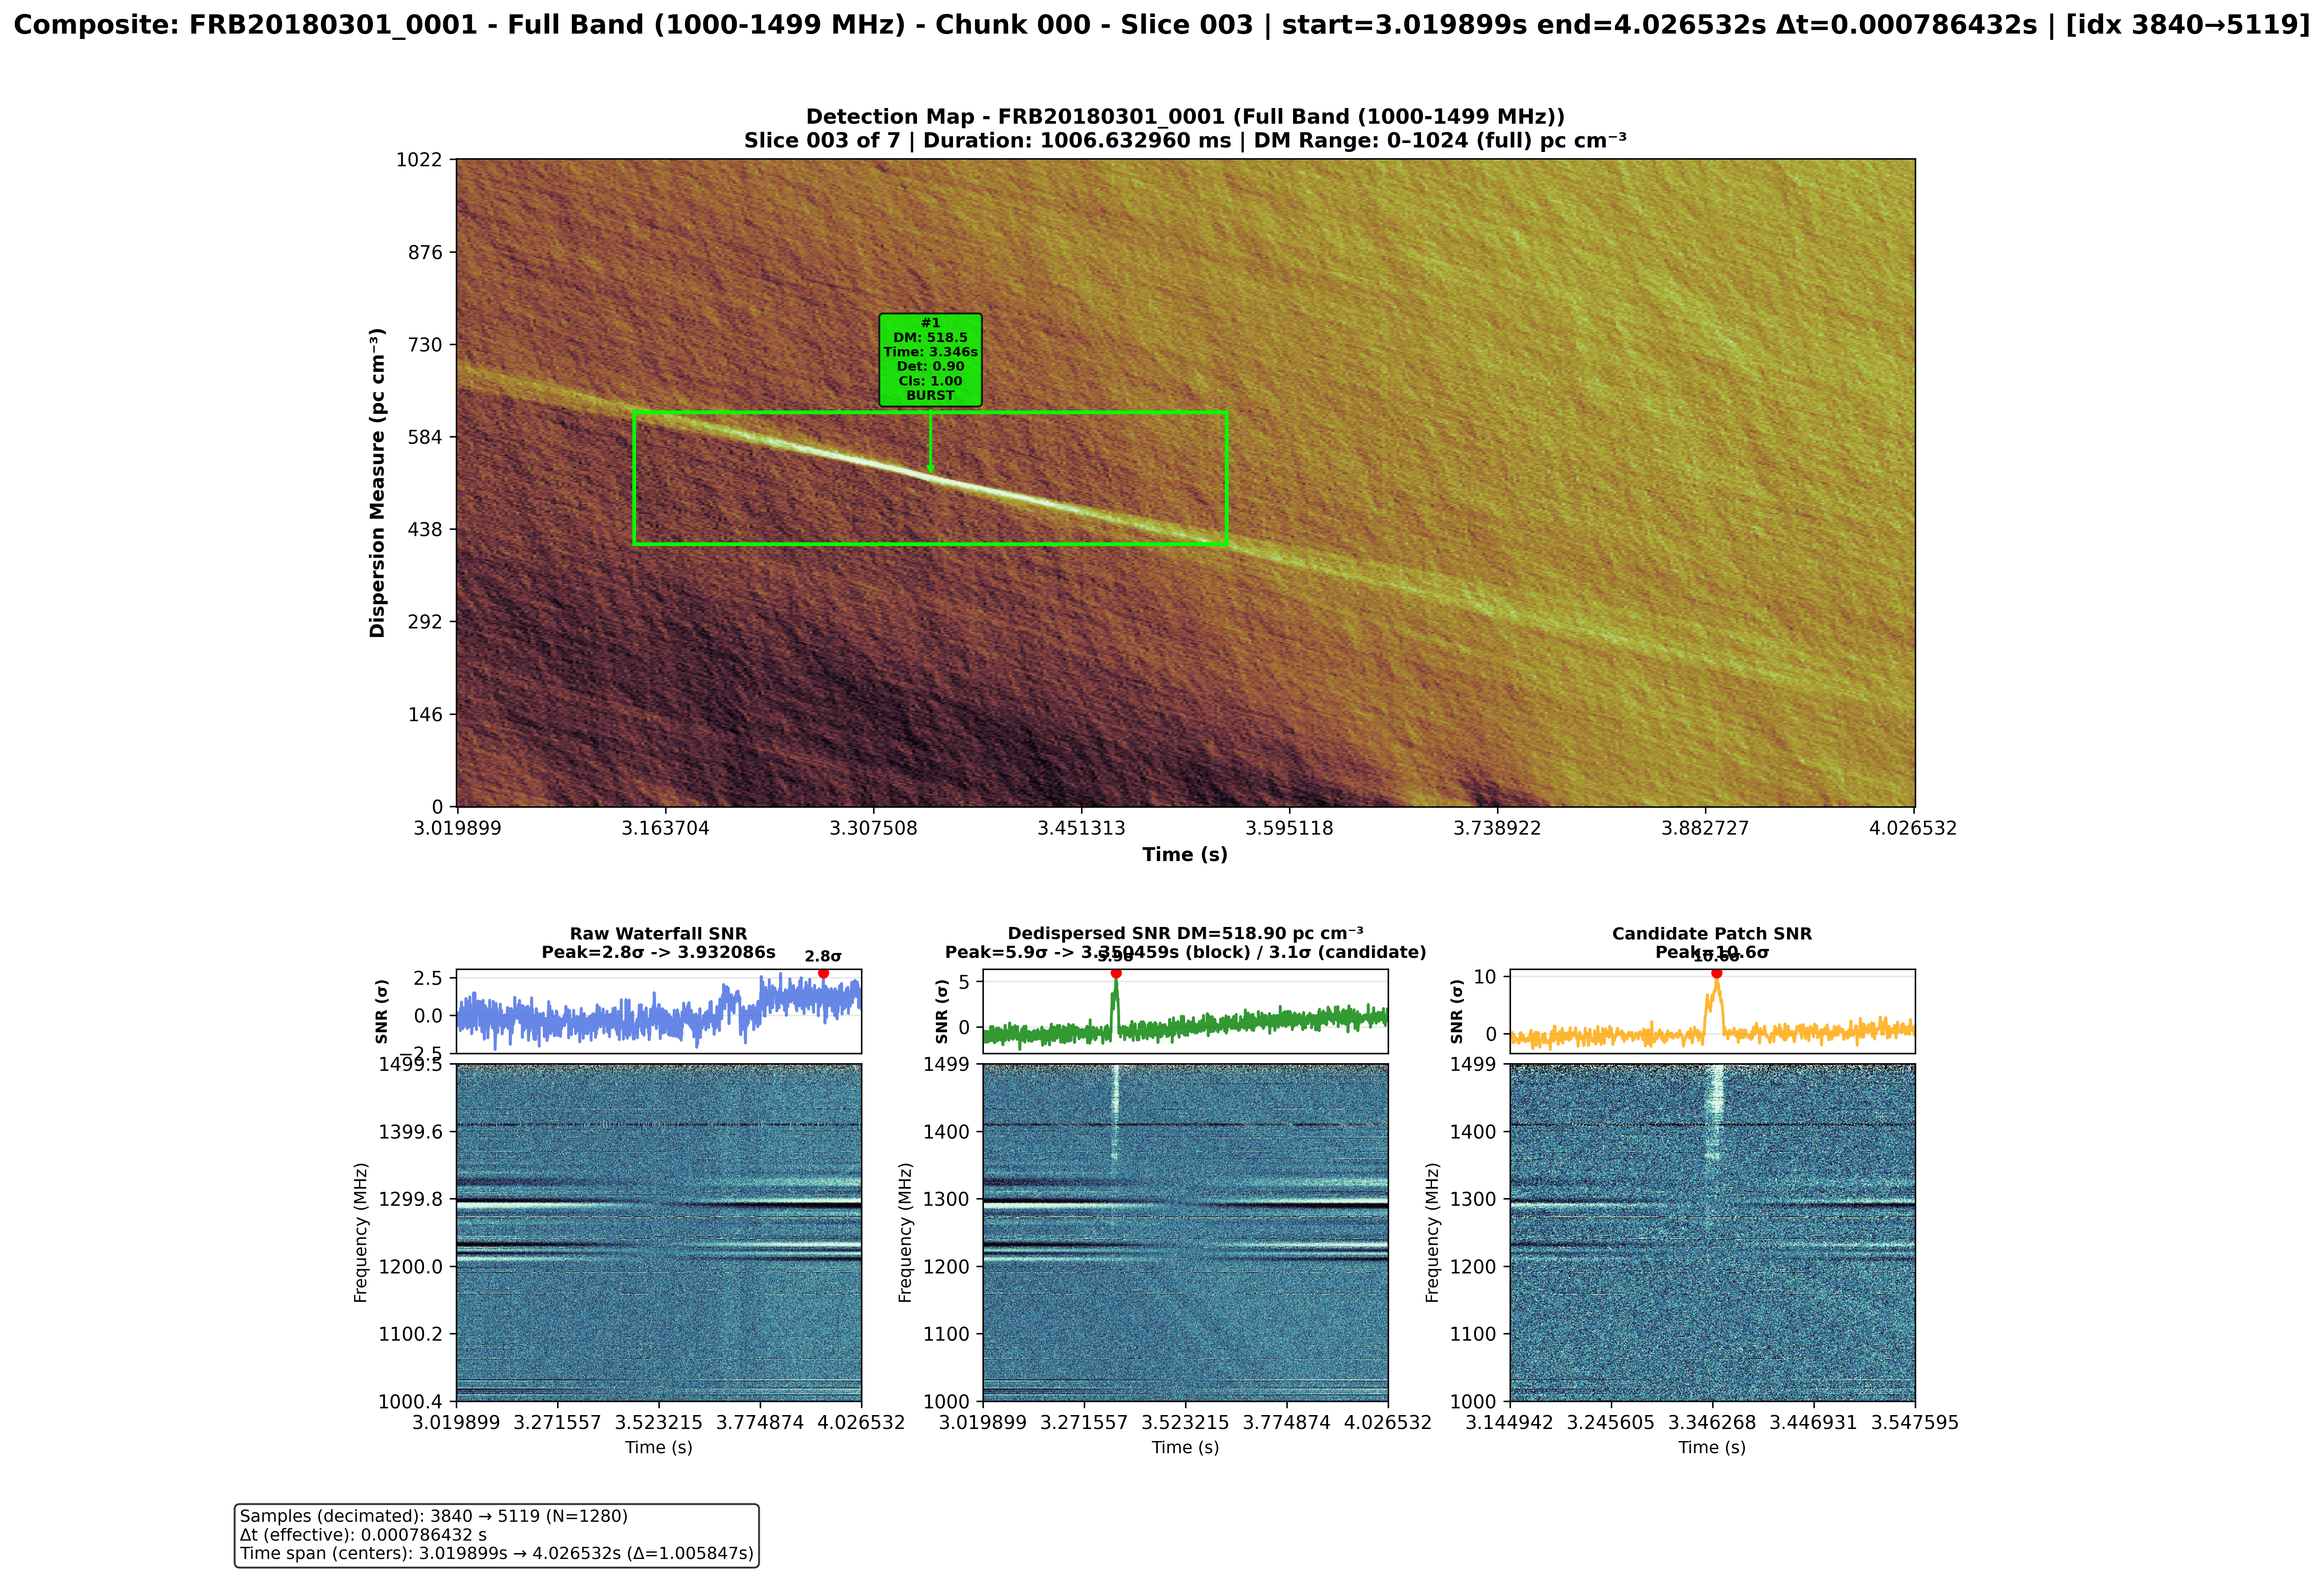
\includegraphics[width=\textwidth]{figures/FRB20180301_0001_slice003.png}
    \caption[Detección FRB (FAST-FREX)]{Detección de un Fast Radio Burst (FRB) del dataset de entrenamiento FAST-FREX. El panel superior muestra el mapa de dispersión (DM vs. Tiempo) con el evento resaltado. Los paneles inferiores presentan el SNR en cascada crudo, el SNR dedispersado y el SNR del parche candidato, confirmando una detección robusta con un SNR de 5.9$\sigma$.}
    \label{fig:frb20180301_0001_slice003}
\end{figure}

\begin{figure}[H]
    \centering
    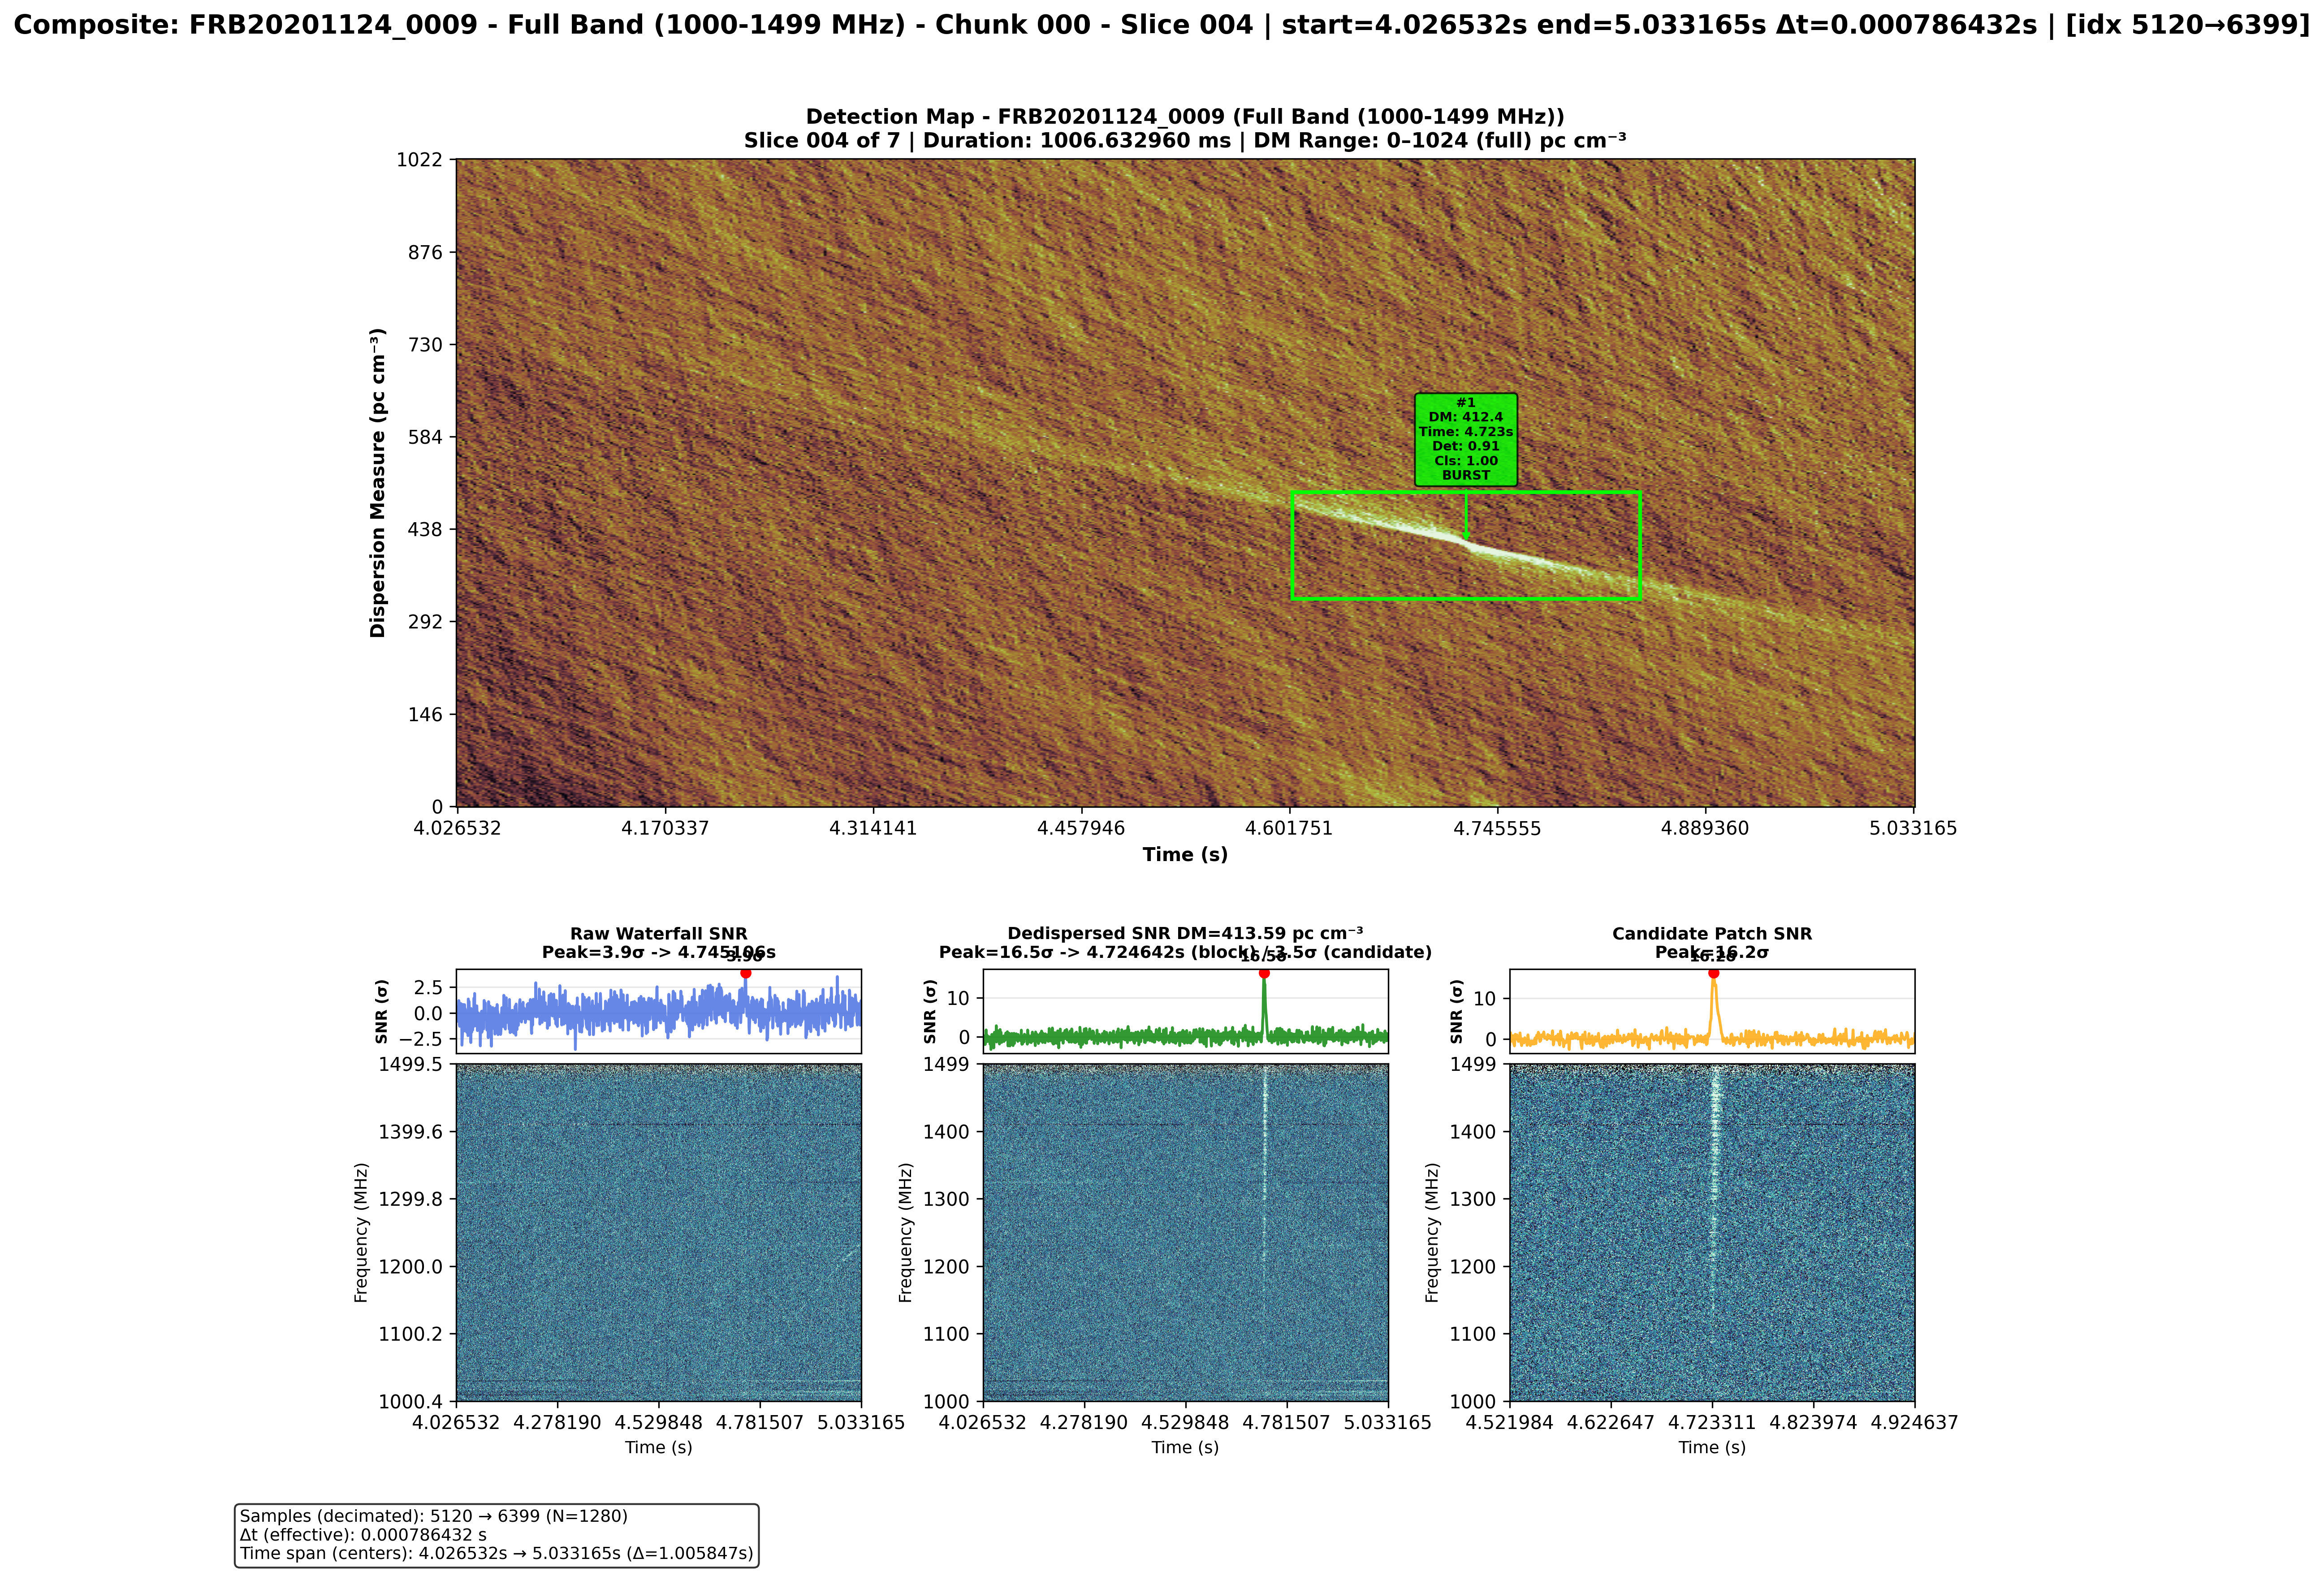
\includegraphics[width=\textwidth]{figures/FRB20201124_0009_slice004.png}
    \caption[Detección FRB adicional (FAST-FREX)]{Detección de un segundo Fast Radio Burst (FRB) del dataset de entrenamiento FAST-FREX. Se observa una detección robusta con SNR de 16.5$\sigma$ después de la dedispersión, confirmando la efectividad del sistema en el dataset de entrenamiento.}
    \label{fig:frb20201124_0009_slice004}
\end{figure}

\subsubsection{Caso 2 - Pulsar B0355+54: Validación de Robustez Temporal y Procesamiento Secuencial}

Una vez establecida la funcionalidad básica del flujo E2E, se procedió a evaluar características arquitectónicas críticas del Componente 1 que diferencian fundamentalmente a DRAFTS++ del prototipo original. Esta validación se centró específicamente en las mejoras de la etapa de preprocesamiento (véase Tabla~\ref{tab:mapeo_validacion_etapas_componente1}), verificando:

\begin{itemize}
    \item \textbf{Contigüidad temporal quirúrgica}: Garantía de que cada slice termina exactamente donde comienza el siguiente, eliminando solapamientos y huecos temporales entre ventanas de procesamiento
    \item \textbf{Arquitectura de streaming por slices}: Procesamiento secuencial de datos en slices con gestión automática de memoria, permitiendo manejar observaciones de duración arbitraria
    \item \textbf{Trazabilidad temporal relativa precisa}: Cálculo exacto de timestamps mediante multiplicación de muestras por resolución temporal, proporcionando localización temporal sub-milisegundo
    \item \textbf{Manejo de discontinuidades}: Detección y gestión automática de interrupciones temporales en datos sin generar errores o artefactos falsos
    \item \textbf{Validación física integrada}: Cálculo automatizado de métricas SNR y verificación de coherencia temporal en cada candidato detectado
\end{itemize}

Para esta validación se utilizó el pulsar de prueba B0355+54\_FB\_20220918, seleccionado por sus características ideales para este propósito:

\begin{itemize}
    \item \textbf{Brightness}: Pulsar sumamente brillante que facilita la detección
    \item \textbf{Periodo de rotación}: 0.156 segundos
    \item \textbf{Duración del archivo}: 117.23 segundos (1 minuto 57 segundos)
    \item \textbf{Pulsos esperados}: 752 pulsos teóricos
\end{itemize}

Los resultados obtenidos fueron altamente satisfactorios:
\begin{itemize}
    \item \textbf{Pulsos detectados}: 732 de 752 esperados (97.3\% de eficiencia)
    \item \textbf{Clasificación}: 718 clasificados como BURSTS, 14 como NO BURSTS
\end{itemize}

\begin{figure}[H]
    \centering
    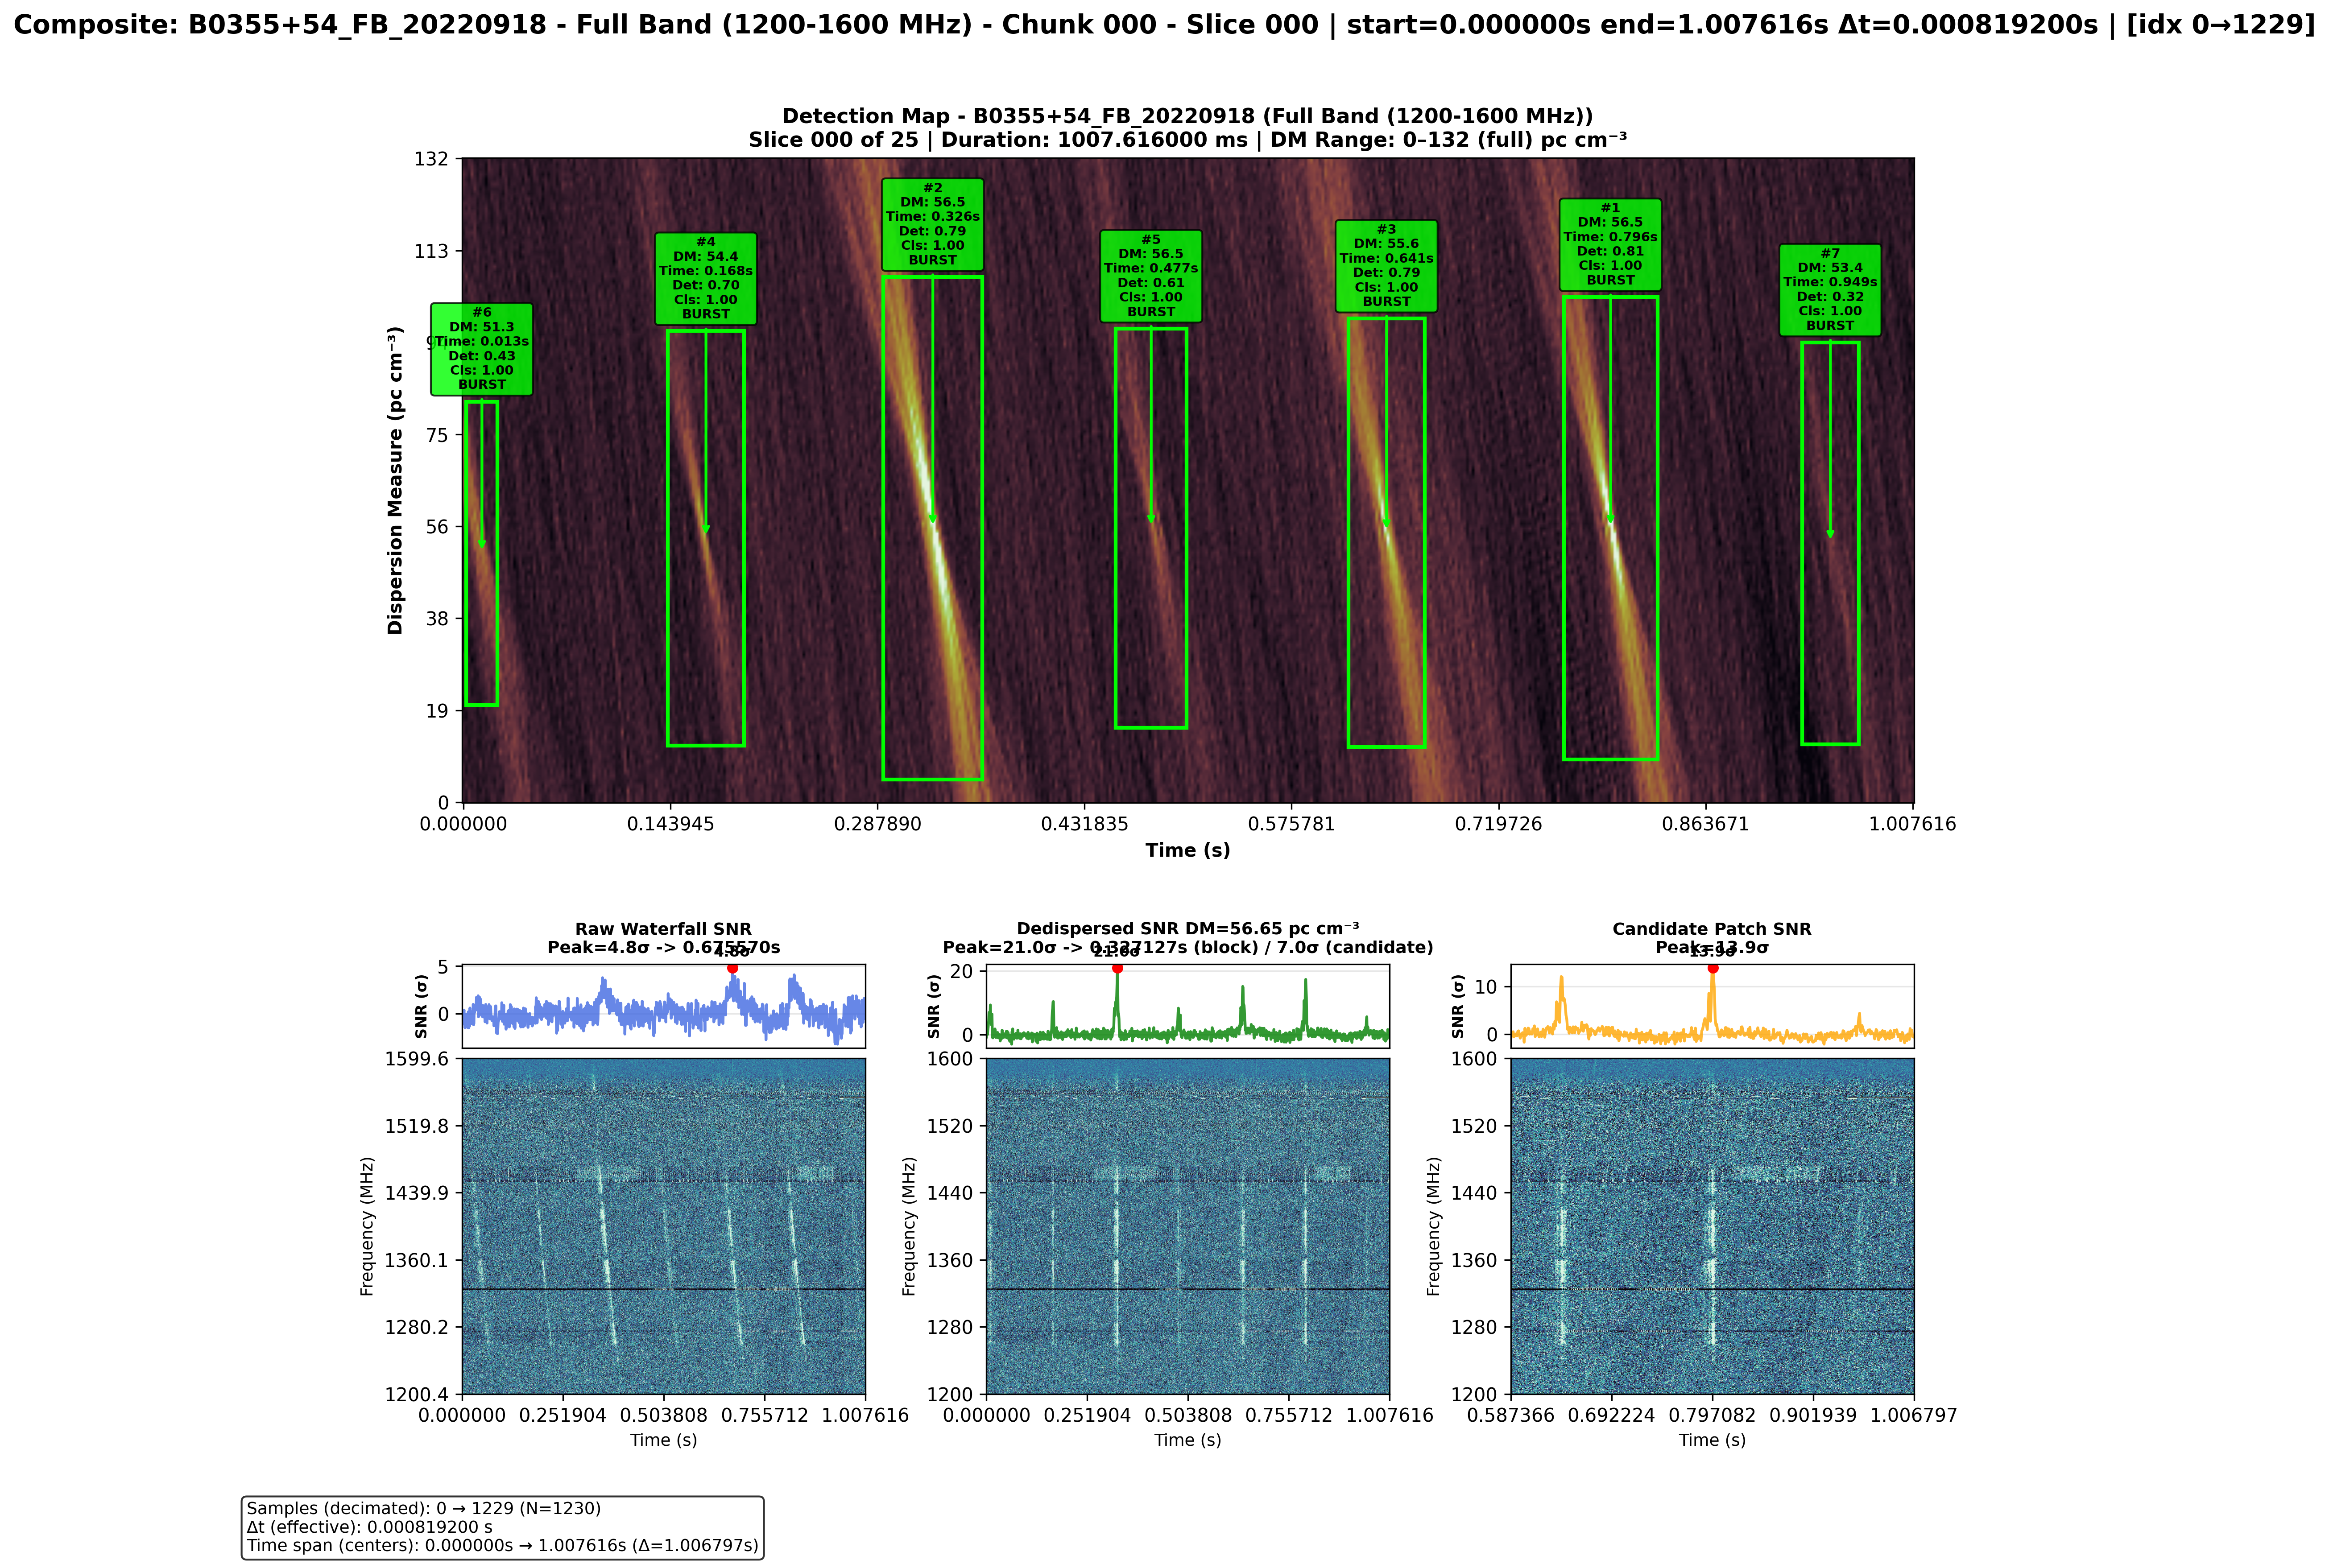
\includegraphics[width=\textwidth]{figures/B0355+54_FB_20220918_slice000.png}
    \caption[Validación continuidad temporal: Slice 000]{Validación de continuidad temporal - Slice 000: Se observan 7 pulsos detectados en el primer segundo de observación, demostrando la capacidad del sistema para detectar eventos periódicos con alta precisión temporal. Todos los pulsos fueron clasificados como BURSTS con scores de clasificación superiores a 0.99.}
    \label{fig:b0355_slice000}
\end{figure}


\begin{figure}[H]
    \centering
    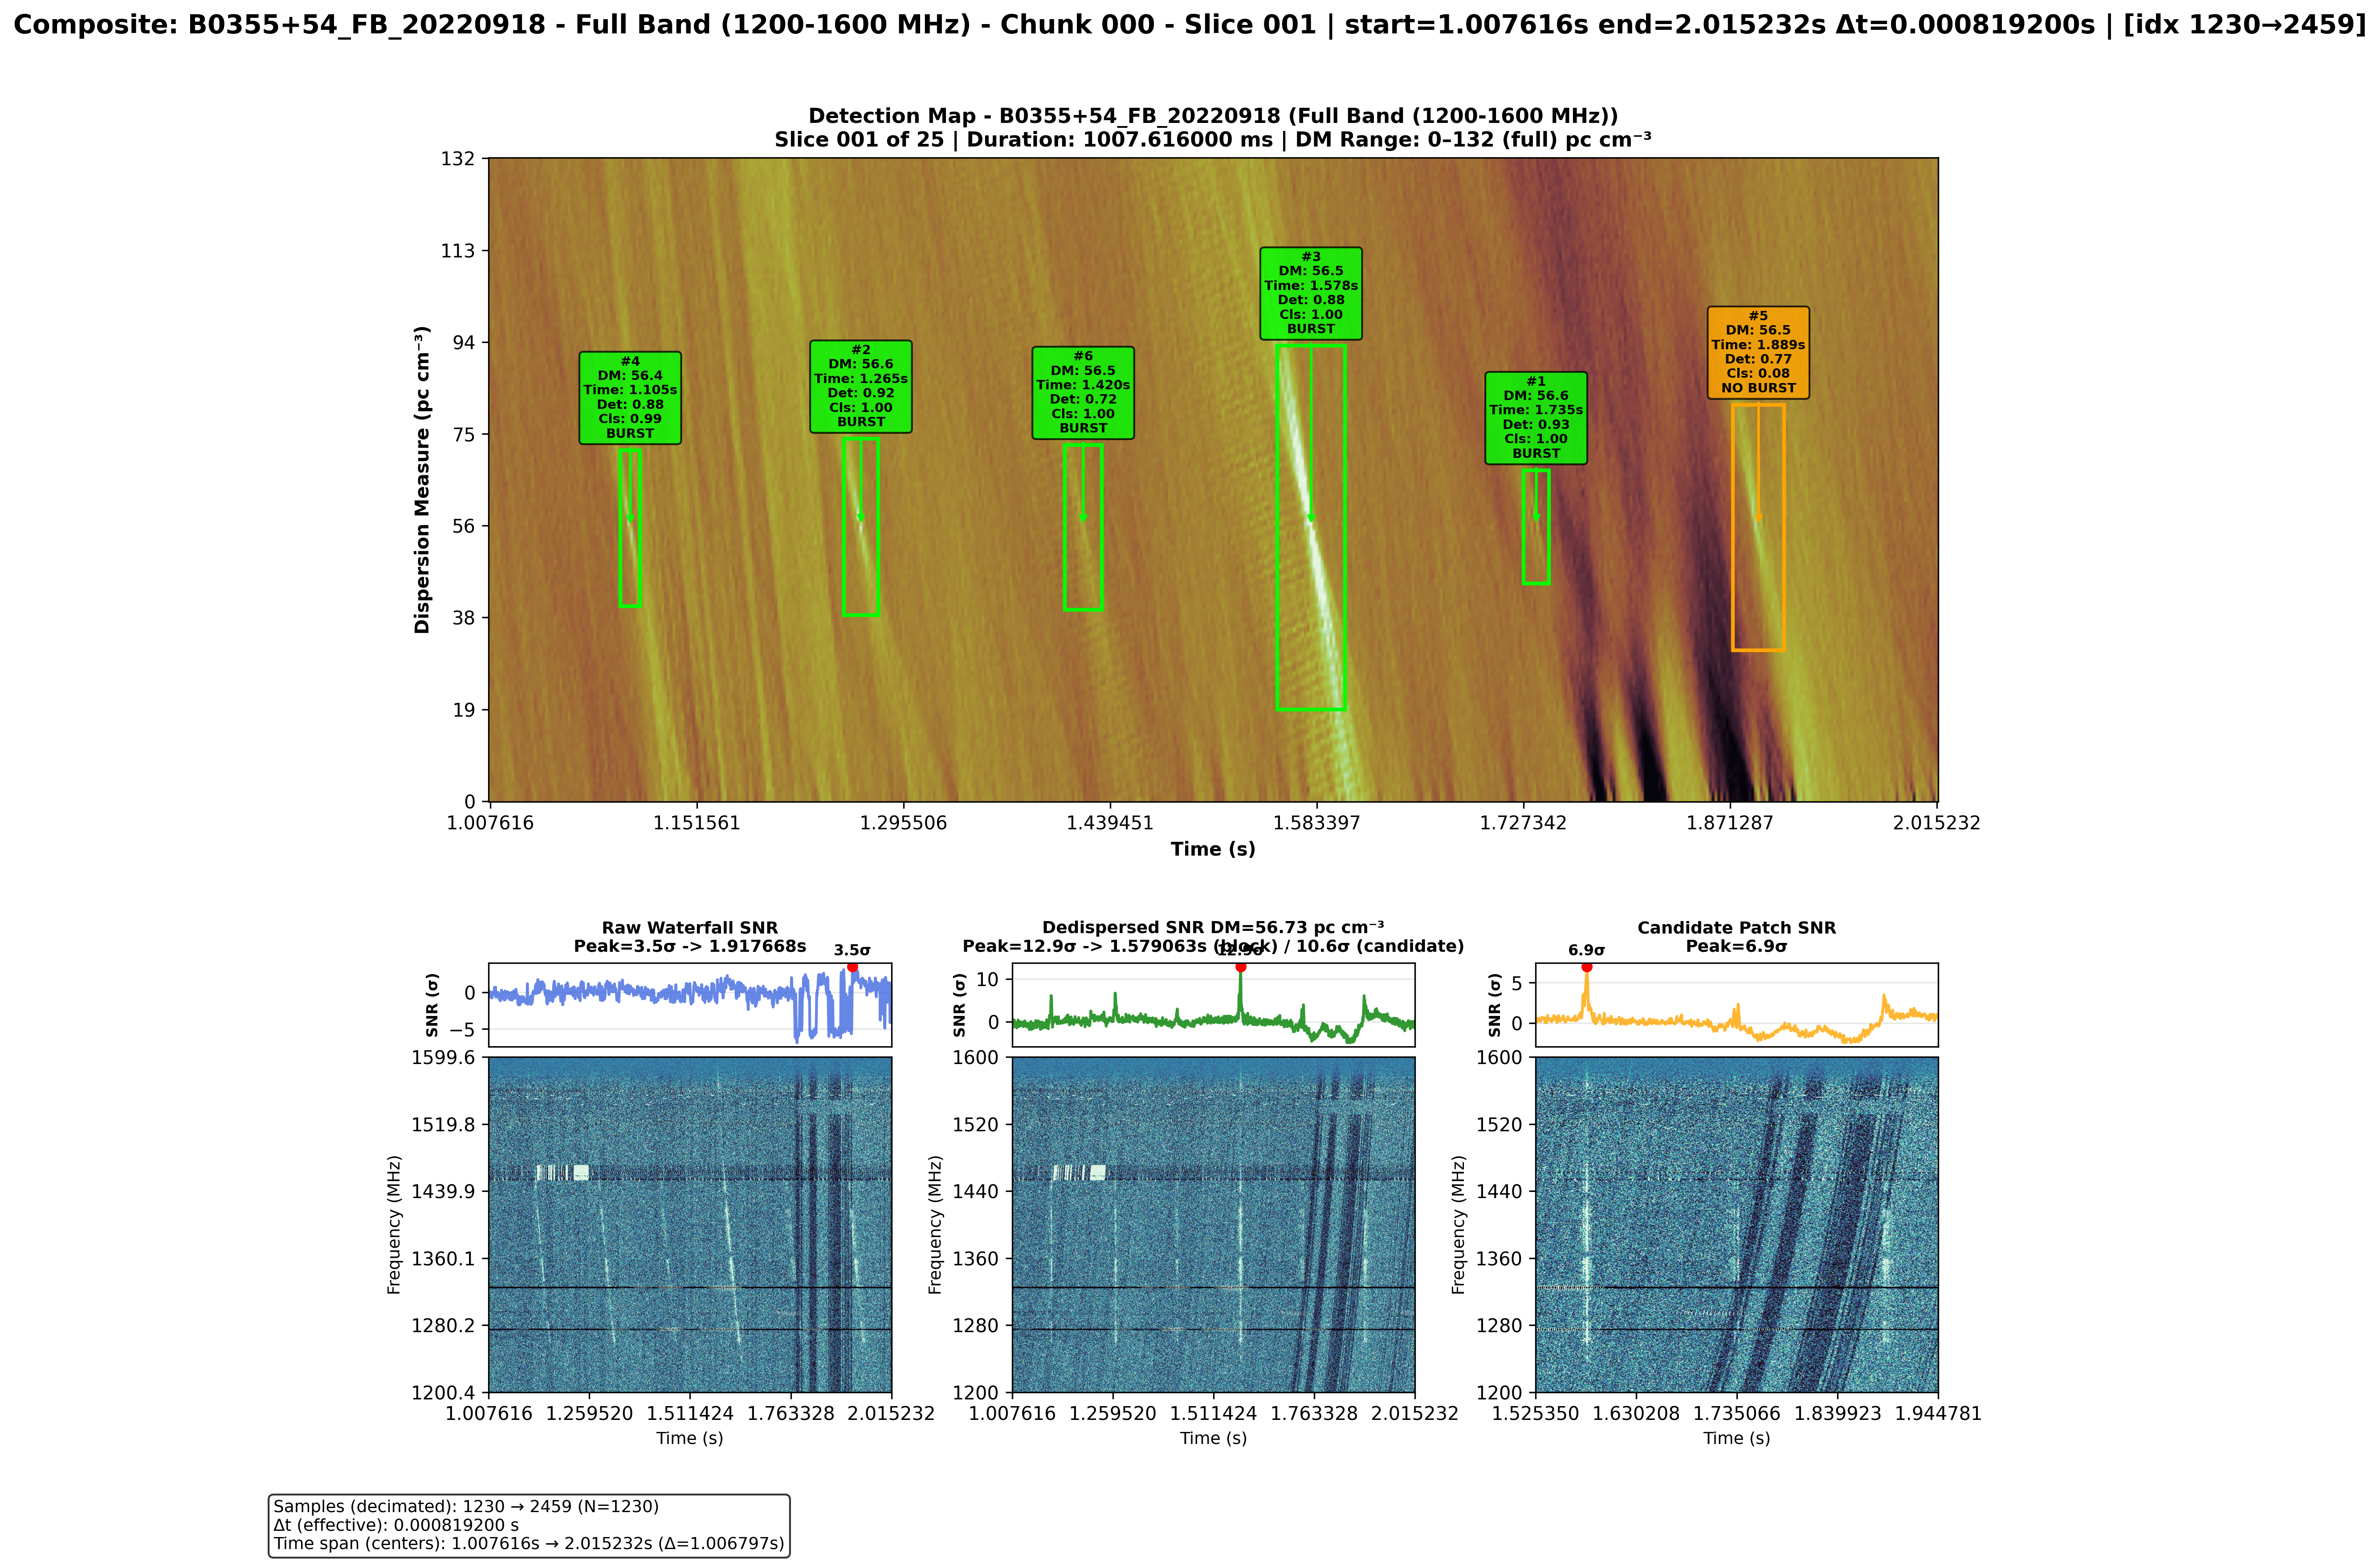
\includegraphics[width=\textwidth]{figures/B0355+54_FB_20220918_slice001.png}
    \caption[Validación continuidad temporal: Slice 001]{Validación de continuidad temporal - Slice 001: Continuidad perfecta en el segundo slice, mostrando 5 pulsos clasificados como BURSTS y 1 como ``NO BURST''. La consistencia en la detección temporal confirma la robustez del sistema de procesamiento por ventanas.}
    \label{fig:b0355_slice001}
\end{figure}

Este resultado confirmó la capacidad del sistema para mantener la continuidad temporal entre ventanas de procesamiento y validó la precisión de las redes de detección pre-entrenadas de DRAFTS en condiciones controladas.

\begin{figure}[H]
    \centering
    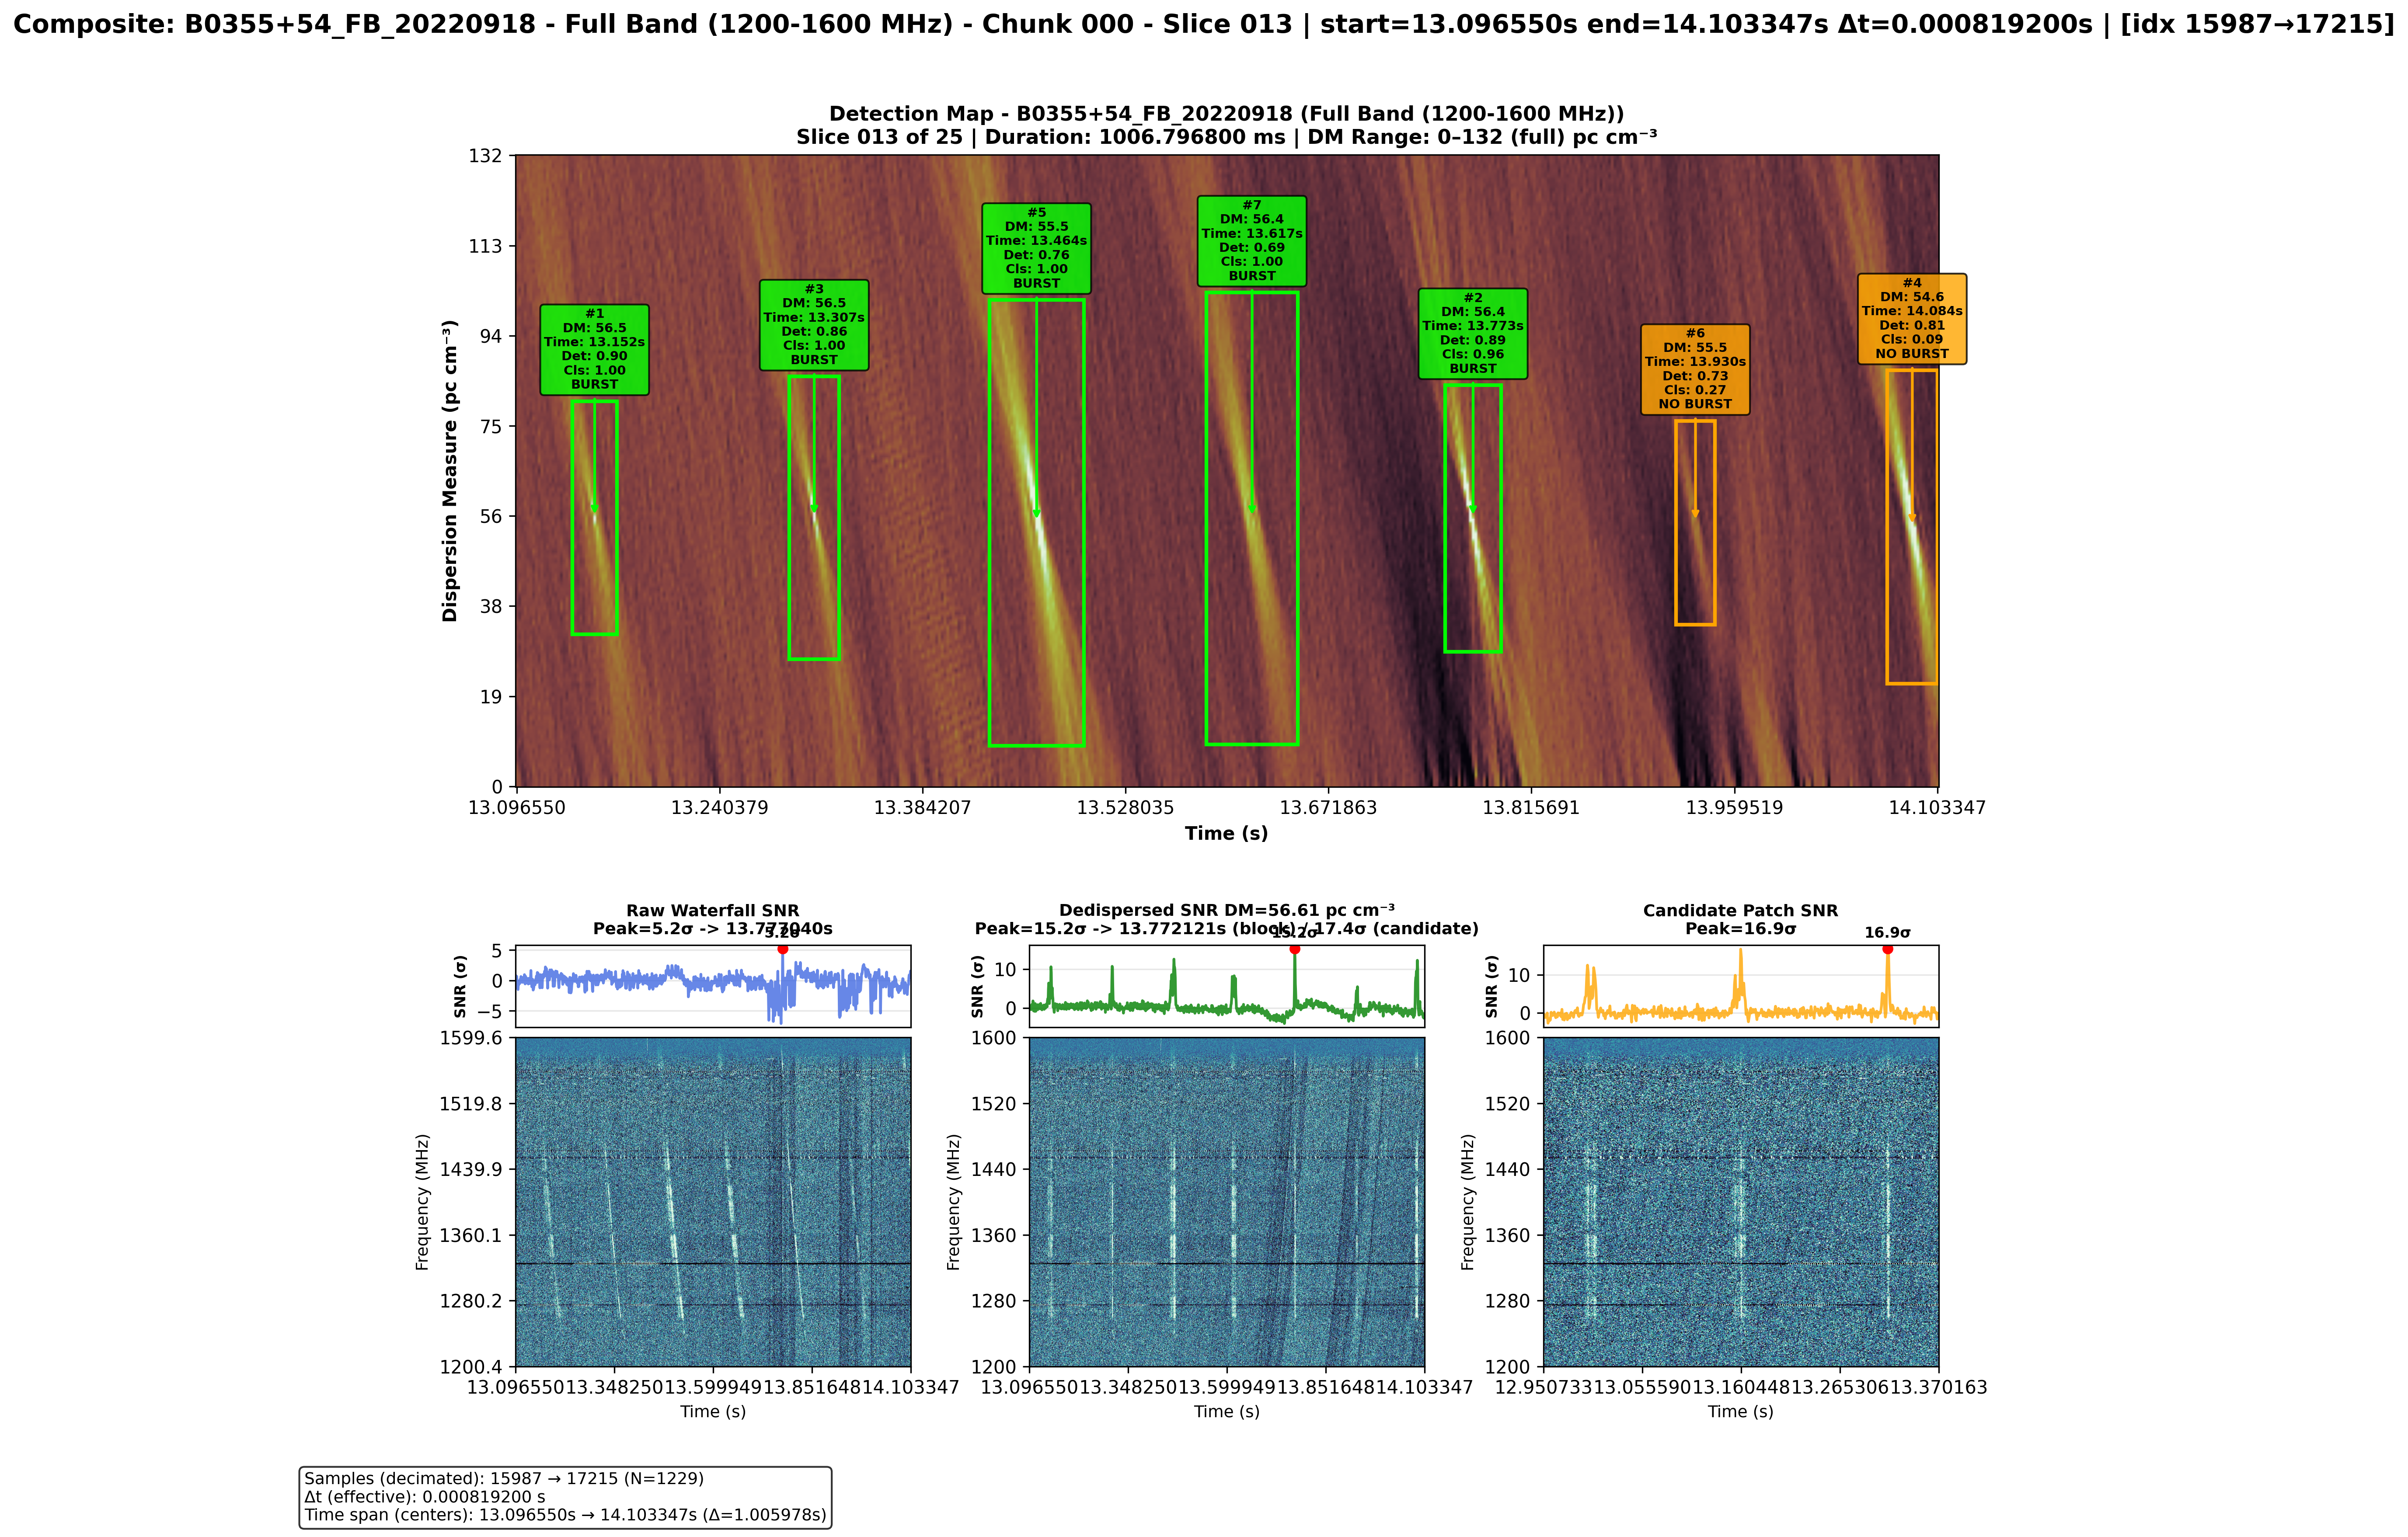
\includegraphics[width=\textwidth]{figures/B0355+54_FB_20220918_slice013.png}
    \caption[Pulso dudoso en la clasificación]{Caso de estudio: Pulso dudoso en la clasificación. El evento \#6 (DM: 55.5, Time: 13.93s) muestra un score de detección alto (0.73) pero un score de clasificación bajo (0.27), resultando en clasificación ``NO BURST''. El evento \#4 (DM: 54.6, Time: 14.08s) presenta un score de detección muy alto (0.81) pero clasificación muy baja (0.09). Esto demuestra la capacidad del sistema para detectar señales ambiguas que requieren revisión manual.}
    \label{fig:b0355_slice013}
\end{figure}

\subsubsection{Caso 3 - FRB 121102: Validación de Escalabilidad E2E y Descubrimiento Científico}

Los casos previos (FAST-FREX y pulsar B0355+54) validaron el flujo E2E básico y la robustez temporal del preprocesamiento, pero operaron sobre archivos de tamaño manejable que cabían completamente en memoria. La validación definitiva del Componente 1 requiere demostrar operación robusta sobre archivos masivos de observaciones reales que exceden ampliamente la memoria disponible, forzando la operación integrada de todas las etapas del pipeline (véase Tabla~\ref{tab:mapeo_validacion_etapas_componente1}): ingesta de archivos multi-gigabyte, chunking con solapamiento controlado, gestión inteligente de memoria RAM/VRAM (módulo core/), procesamiento E2E sin intervención manual, y capacidad de descubrimiento científico genuino.

El dataset del FRB 121102 proporciona este escenario desafiante. Los archivos de observación del telescopio Effelsberg presentan tamaños de varios gigabytes, requiriendo la operación integrada de todas las mejoras arquitectónicas: sistema de chunking con solapamiento controlado, planificación dinámica de recursos, gestión inteligente de memoria GPU con fallback automático a CPU, y continuidad temporal quirúrgica entre chunks. Adicionalmente, este dataset permite validación científica rigurosa mediante comparación directa con resultados publicados en literatura.

Se utilizaron 6 archivos de observación, correspondientes a los reportados por \cite{cruces2020frb121102} en su estudio de periodicidad y comportamiento temporal. Esta referencia proporciona ground truth de 24 eventos confirmados, permitiendo evaluar recall del sistema mediante comparación directa. 

El pipeline procesó exitosamente los 6 archivos de observación, detectando 41 eventos distribuidos a lo largo de las sesiones. El sistema recuperó la totalidad de los 24 bursts reportados por Cruces et al. (2021), logrando Recall = 100\% sobre eventos conocidos. Este resultado confirma que el sistema de chunking no introduce pérdida de sensibilidad: eventos cercanos a bordes de chunks fueron detectados correctamente gracias al solapamiento controlado implementado.

Adicionalmente, el sistema identificó 17 candidatos nuevos no reportados en literatura. La validación científica independiente confirmó 2 de estos eventos como bursts genuinos (Figuras \ref{fig:new_event_3096} y \ref{fig:new_event_3102}), mientras que los 15 restantes permanecen como candidatos prometedores pendientes de análisis adicional. Los eventos confirmados muestran SNR de 6.3$\sigma$ y 12.0$\sigma$ respectivamente, con DM~564 pc cm$^{-3}$ consistente con la fuente, y morfología temporal característica de FRB 121102.

% Las detecciones completas se documentan en Anexo A: bursts confirmados por literatura (Tabla \ref{tab:anexo_confirmed_bursts}), nuevos eventos confirmados (Tabla \ref{tab:anexo_new_confirmed_bursts}), y candidatos pendientes (Tabla \ref{tab:anexo_candidate_bursts}). El histograma de distribución temporal (Figura \ref{fig:frb121102_histogram}) muestra concentración de eventos en archivos 3098 y 3100, consistente con ventanas de actividad del repetidor.

\begin{figure}[H]
    \centering
    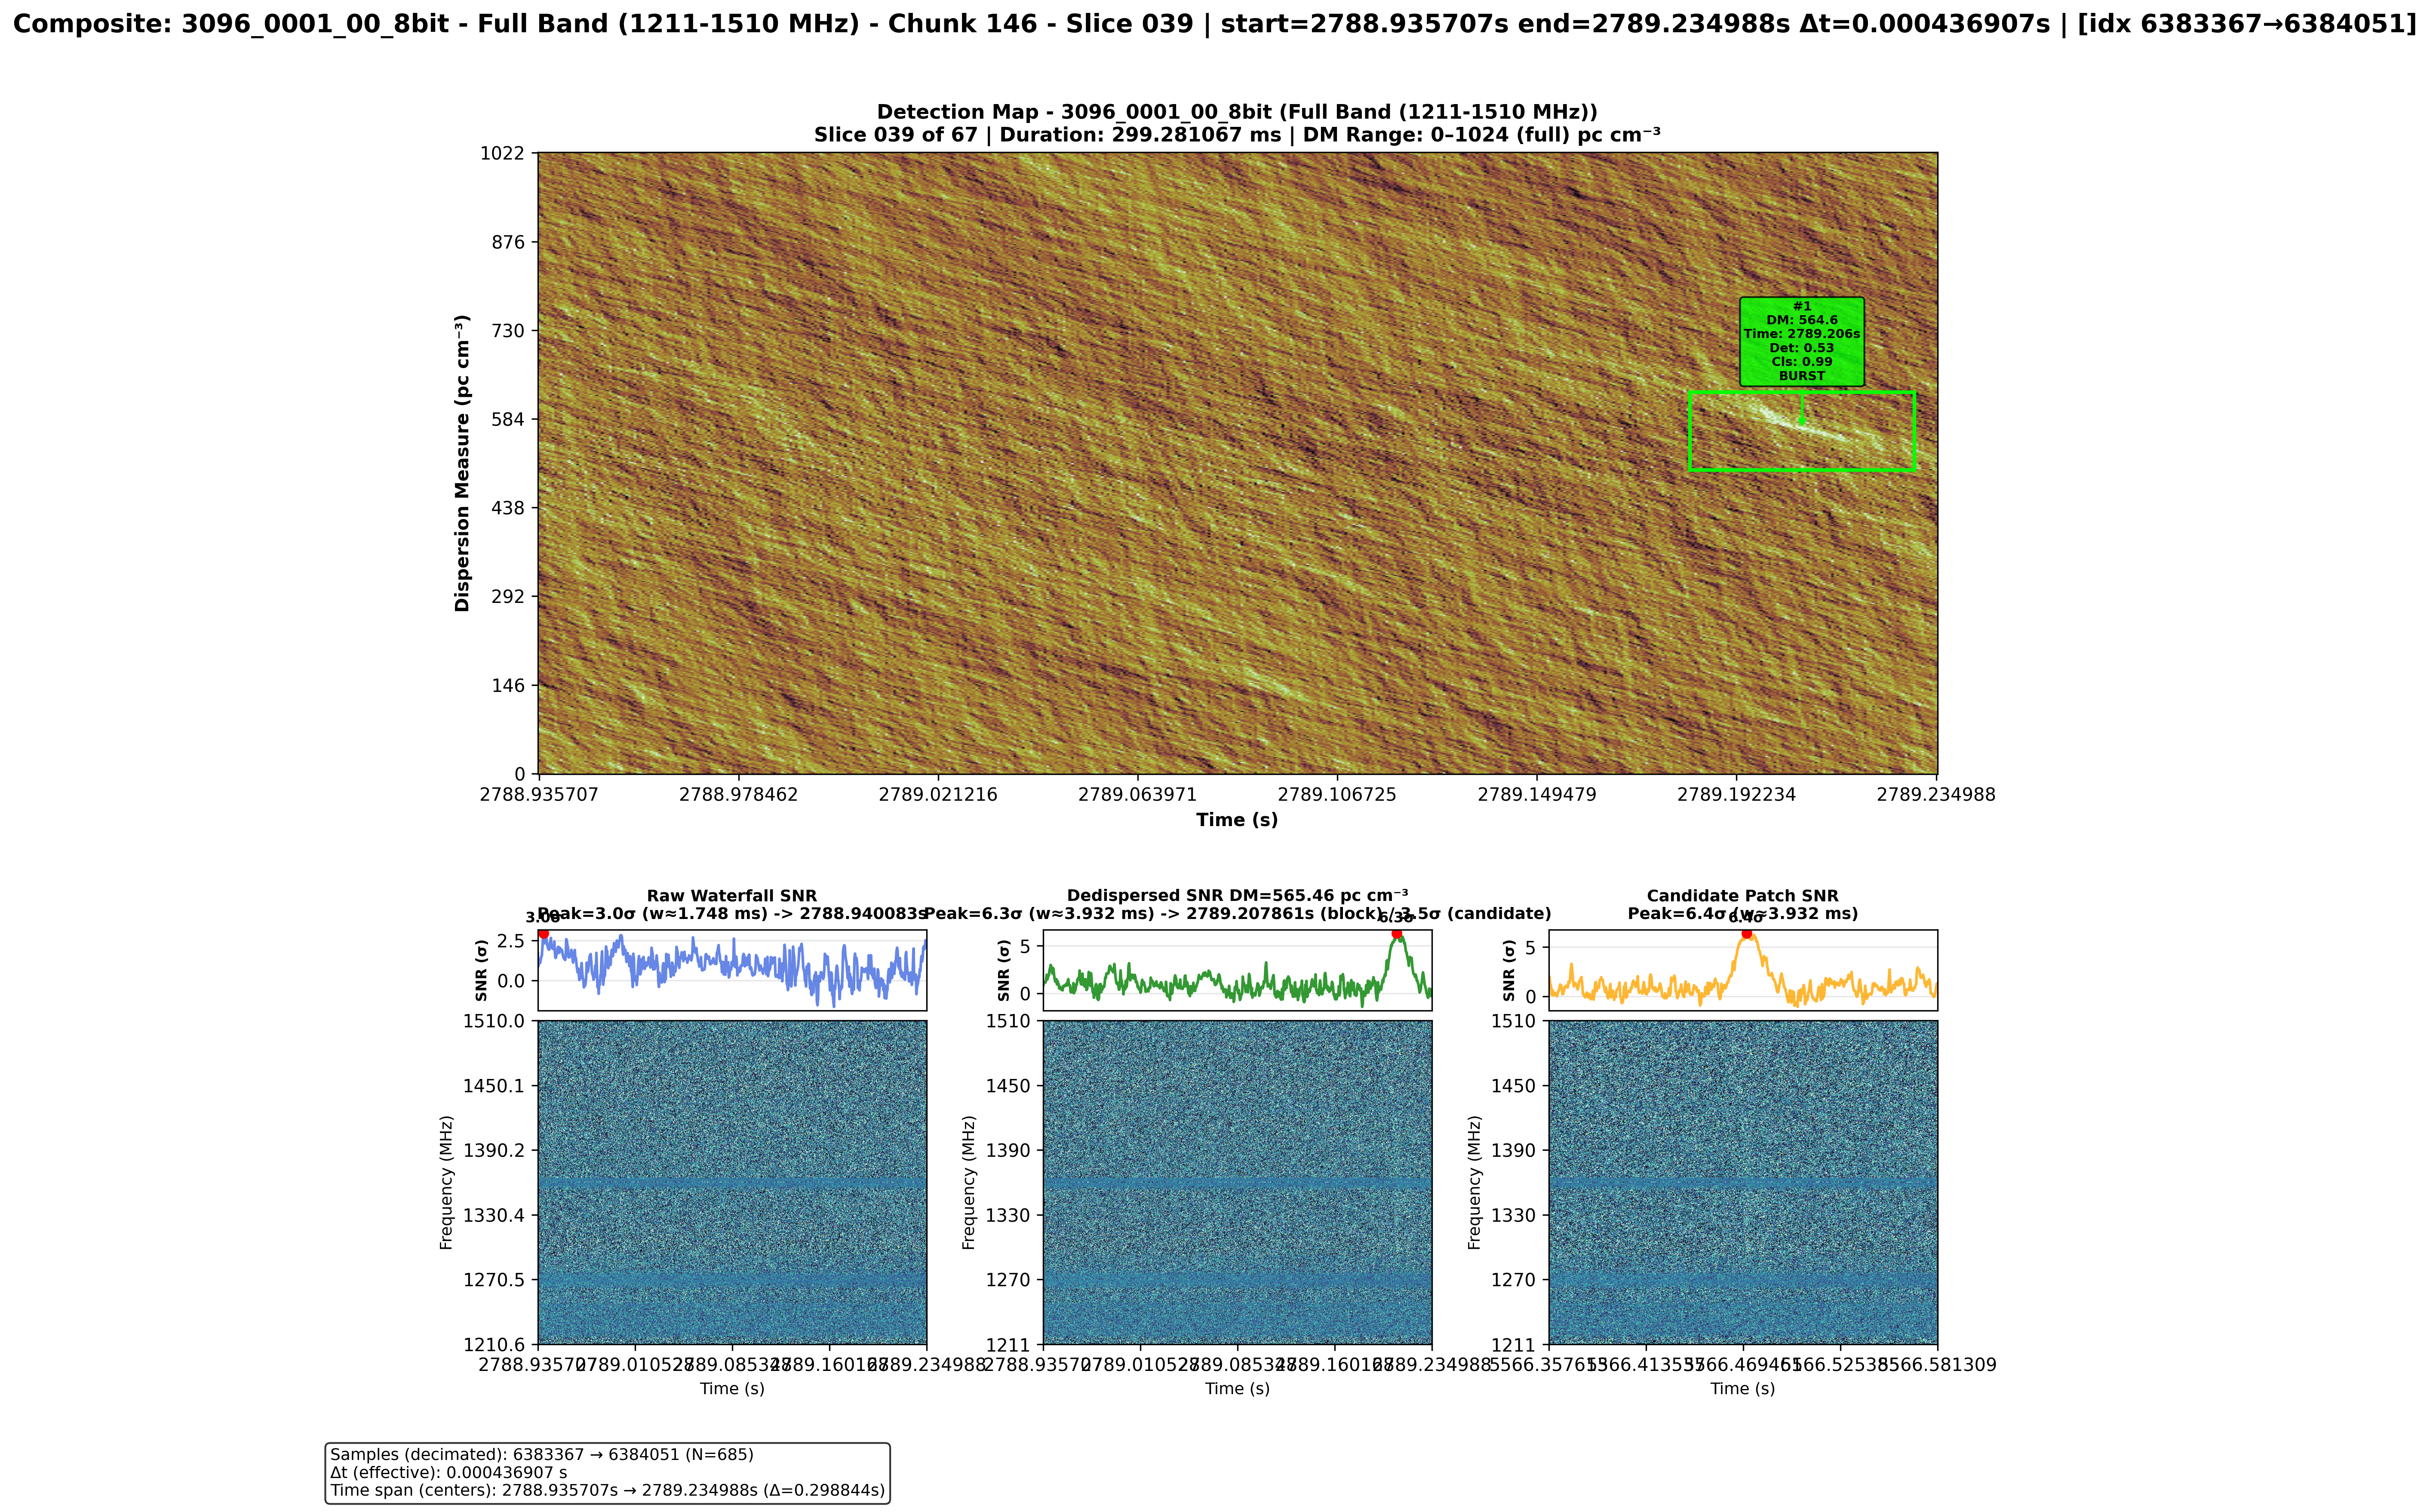
\includegraphics[width=\textwidth]{figures/3096_0001_00_8bit_slice039.png}
    \caption[FRB121102: nuevo evento confirmado (3096\_...\_slice039)]{Primer nuevo evento confirmado de FRB121102 detectado por DRAFTS++ en el archivo 3096\_0001\_00\_8bit, slice 039. El evento muestra DM=563.6 pc cm$^{-3}$ y Time=2421.559296s, con un SNR de 6.3$\sigma$ después de la dedispersión. La detección fue 100\% confirmada por el grupo de astrónomos colaboradores. \textit{Fuente: Elaboración propia}.}
    \label{fig:new_event_3096}
\end{figure}

\begin{figure}[H]
    \centering
    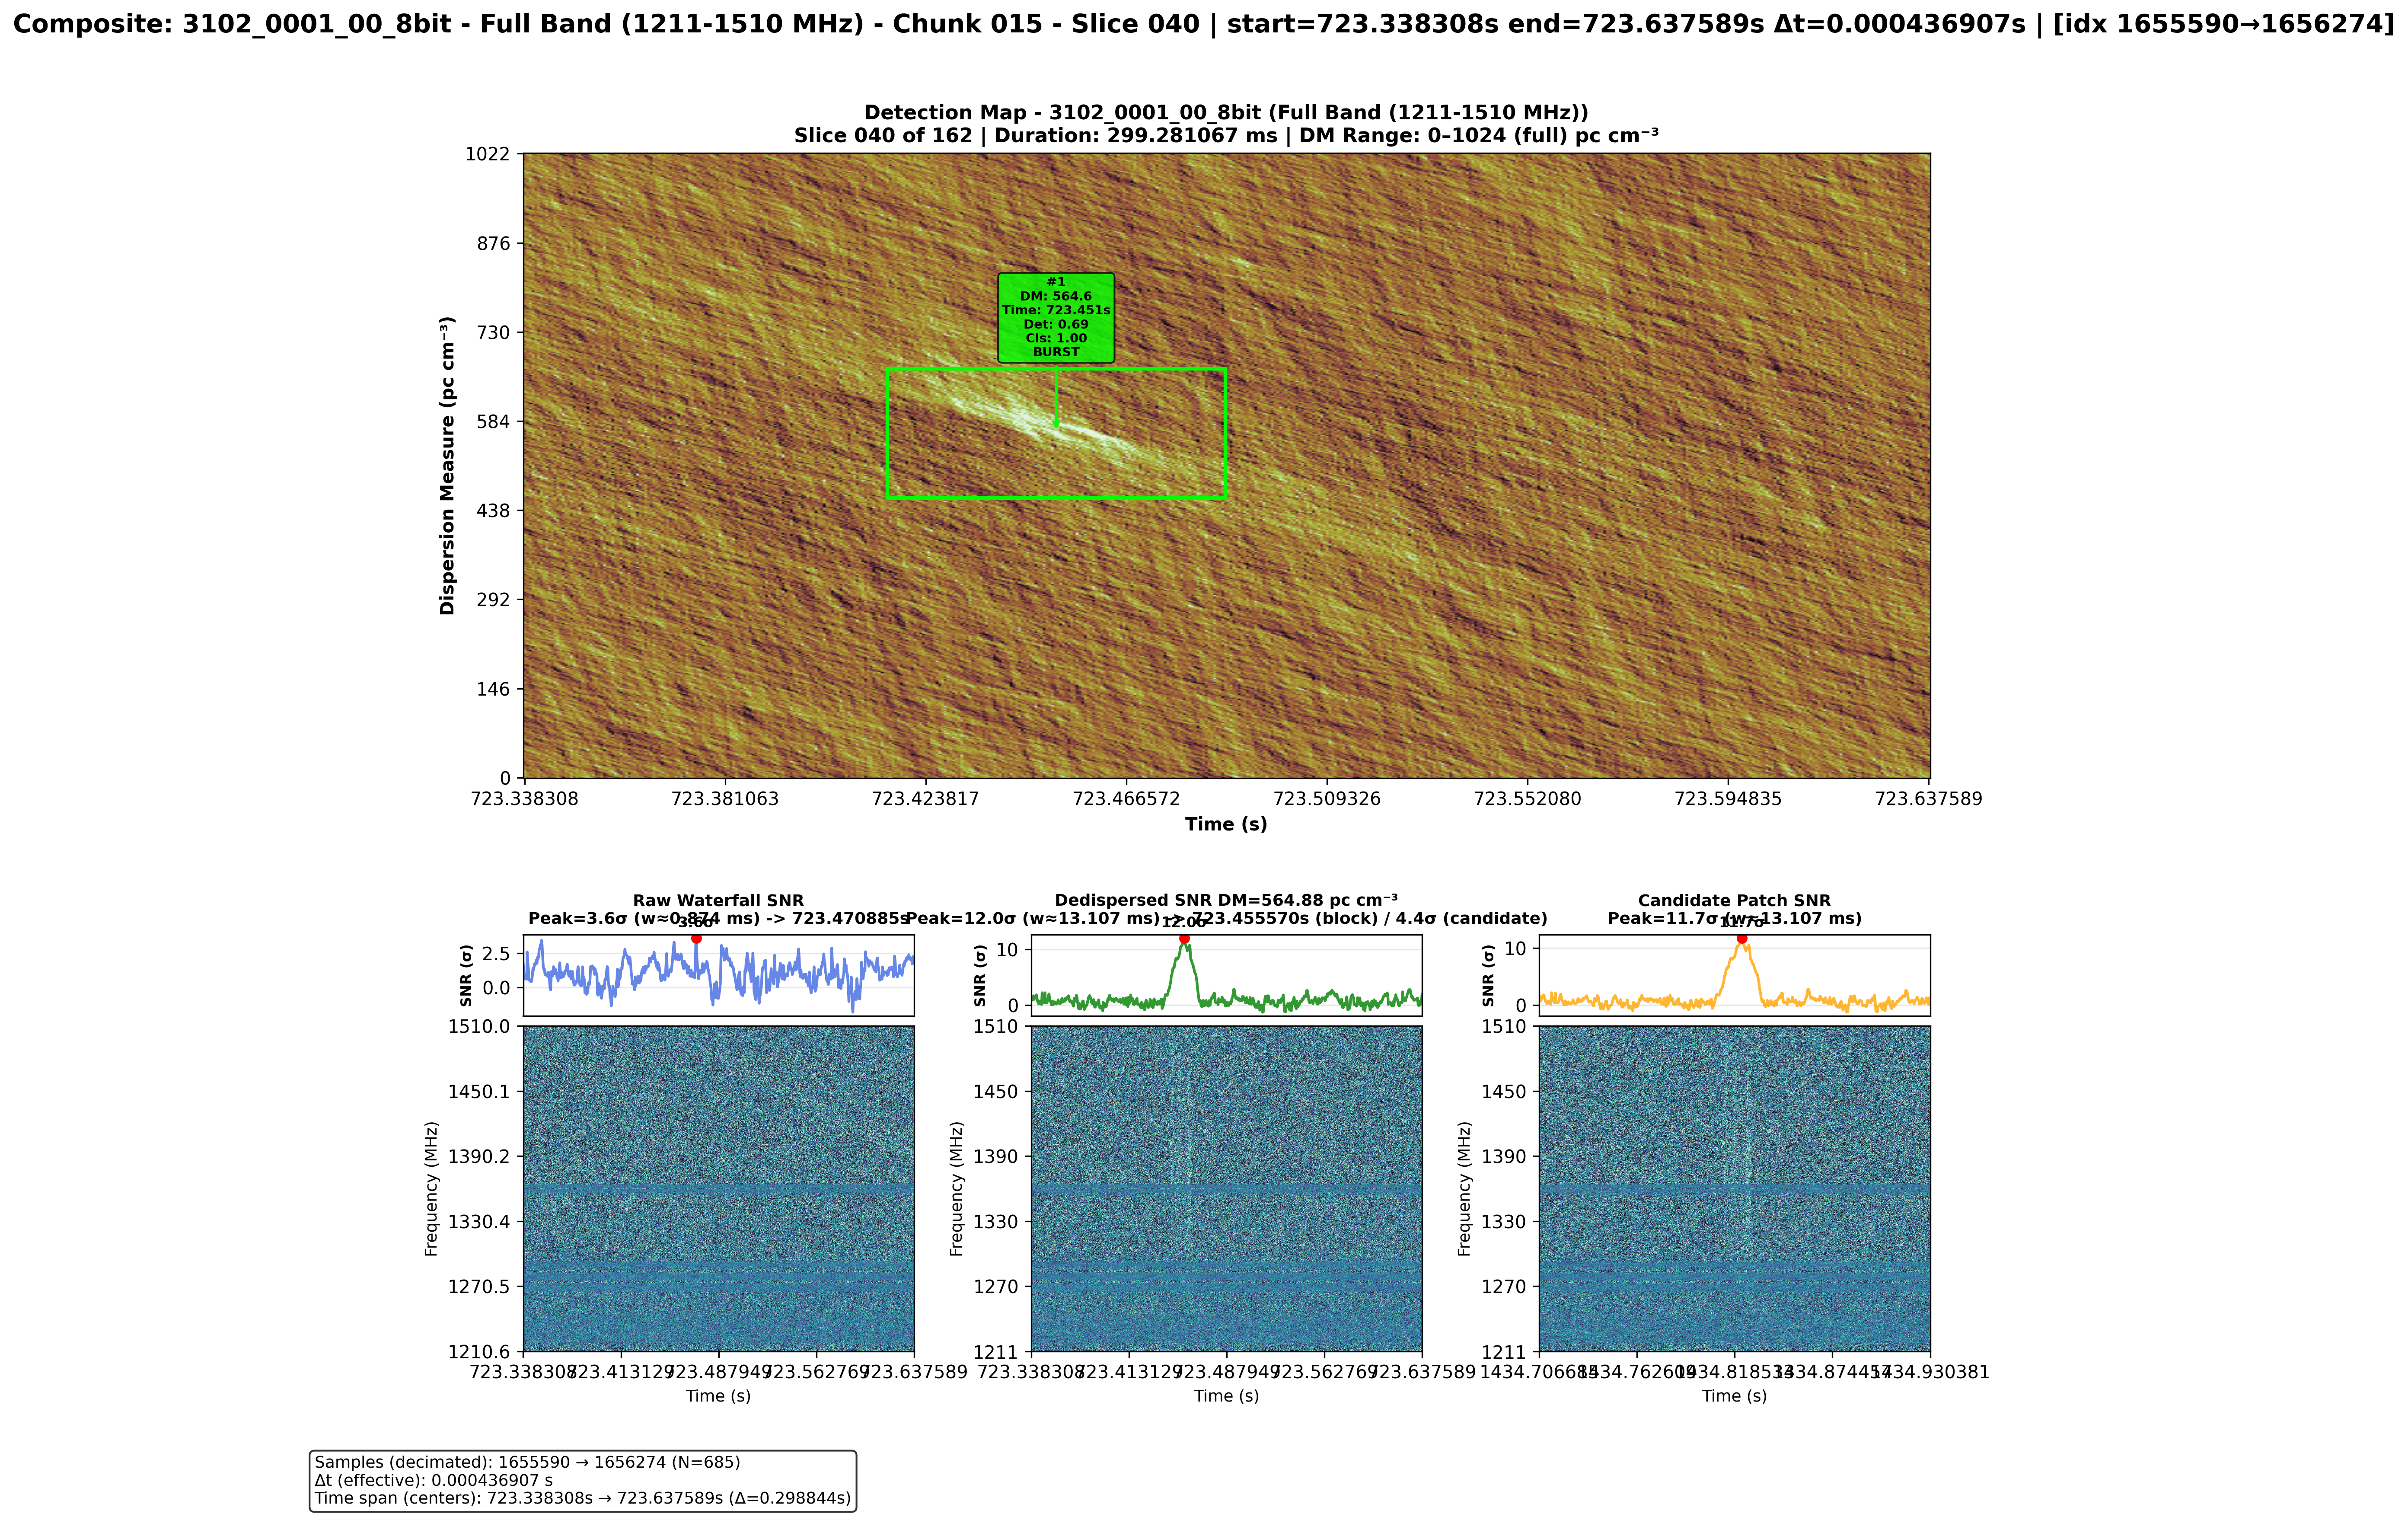
\includegraphics[width=\textwidth]{figures/3102_0001_00_8bit_slice040.png}
    \caption[FRB121102: nuevo evento confirmado (3102\_...\_slice040)]{Segundo nuevo evento confirmado de FRB121102 detectado por DRAFTS++ en el archivo 3102\_0001\_00\_8bit, slice 040. El evento muestra DM=564.88 pc cm$^{-3}$ y Time=723.455399s, con un SNR de 12.0$\sigma$ después de la dedispersión. Este evento representa uno de los bursts más brillantes detectados en el dataset y fue 100\% confirmado por el grupo de astrónomos colaboradores. \textit{Fuente: Elaboración propia}.}
    \label{fig:new_event_3102}
\end{figure}

% \begin{figure}[H]
%     \centering
%     \includegraphics[width=0.8\textwidth]{figures/frb121102_detection_histogram.png}
%     \caption[Histograma de detecciones FRB121102]{Distribución temporal de detecciones por archivo de observación. Morado: bursts confirmados por literatura; Celeste: nuevos candidatos sin confirmar; Verde: nuevos eventos confirmados. La concentración en archivos 3098 y 3100 es consistente con ventanas de actividad del repetidor. \textit{Fuente: Elaboración propia}.}
%     \label{fig:frb121102_histogram}
% \end{figure}

Los resultados validan integralmente el Componente 1. El pipeline procesó exitosamente archivos multi-gigabyte sin errores de memoria ni degradación de rendimiento, operando sin intervención manual desde ingesta hasta visualización. El recall perfecto (26/26 eventos detectados: 24 de literatura + 2 nuevos confirmados) demuestra que el sistema de chunking con solapamiento controlado no introduce puntos ciegos temporales, validando la continuidad temporal quirúrgica implementada. El descubrimiento de 2 nuevos bursts confirmados demuestra capacidad de descubrimiento científico genuino.

\subsection{VALIDACIÓN DEL COMPONENTE 2: DRAFTS++ - Extensión a Alta Frecuencia - Cuatro Líneas de Investigación}

La validación del Componente 2 examina la efectividad de DRAFTS++ en el régimen milimétrico (86 GHz), donde la firma dispersiva tradicional se comprime significativamente debido a la dependencia $\Delta t_{\mathrm{ms}} \propto \nu^{-2}$. En este régimen, el patrón bow-tie característico de FRBs en bajas frecuencias (1.4 GHz) colapsa, desafiando a detectores entrenados en firmas dispersivas desarrolladas.

Para todas las líneas de investigación se valido utilizando observaciones del radiotelescopio ALMA del magnetar del Centro Galáctico PSR J1745-2900 a 86 GHz, proporcionadas por \cite{veracasanova2025}. Este dataset constituye ground truth mediante 8 pulsos confirmados independientemente con PRESTO (Tabla~\ref{tab:veracasanova_reference}), permitiendo evaluación objetiva de cada estrategia.

\begin{table}[H]
    \centering
\caption{Ground truth: Pulsos del magnetar PSR J1745-2900 reportados por Vera-Casanova et al. (2025), utilizados para validación de todas las líneas de investigación.}
    \label{tab:veracasanova_reference}
\small
    \begin{tabular}{|c|c|}
        \hline
\textbf{File} & \textbf{Timestamp (s)} \\
        \hline
        142\_0003 & 39.977 \\
142\_0006 & 10.882, 25.829 \\
        153\_0006 & 23.444 \\
230\_0002 & 2.3, 17.395 \\
        230\_0003 & 36.548 \\
        242\_0005 & 44.919 \\
        \hline
\multicolumn{2}{|c|}{Total: 8 pulsos confirmados} \\
\hline
    \end{tabular}
\end{table}

Las métricas de evaluación son estándar: Recall, que mide sensibilidad (fracción de pulsos genuinos detectados), Precision, que cuantifica especificidad (proporción de detecciones correctas), y F1-score que sintetiza el balance entre ambas. Los resultados se complementan con análisis de casos representativos que ilustran modos de éxito y falla de cada estrategia.

\subsubsection{Línea 1: Validación de Transferibilidad del Pipeline Clásico mediante Adaptación Paramétrica}

Esta línea establece el baseline de rendimiento del pipeline clásico (CenterNet + ResNet18) en alta frecuencia sin modificaciones arquitecturales, evaluando si ajustes paramétricos simples pueden compensar la compresión del bow-tie. El experimento compara dos configuraciones de umbral de detección: conservadora (DET\_PROB = 0.3, optimizada en bajas frecuencias) y sensible (DET\_PROB = 0.05, factor x6 más permisivo), aislando el efecto del umbral sobre sensibilidad y especificidad.

Los resultados revelaron comportamiento bimodal dramático. Con el umbral estándar (DET\_PROB = 0.3), el sistema falló completamente: ninguno de los 8 pulsos de referencia fue detectado. Este resultado confirma que modelos optimizados para bow-ties desarrollados no transfieren directamente a regímenes comprimidos, independientemente de la calidad del entrenamiento original.

Al reducir el umbral en factor x6 (DET\_PROB = 0.05), el sistema recuperó sensibilidad parcial detectando 7/8 pulsos (Recall = 87.5\%), pero introdujo aproximadamente 12 candidatos espurios, degradando la precisión a 36.8\%. El F1-score de 51.8\% refleja el trade-off fundamental entre sensibilidad y especificidad inherente a la adaptación paramétrica: ajustar el umbral desplaza el punto de operación en la curva ROC pero no expande el dominio de representación del modelo. La Tabla \ref{tab:comparacion_umbrales_linea1} sintetiza estas métricas.

\begin{table}[H]
    \centering
    \caption{Rendimiento del pipeline clásico adaptado según configuración de umbral. Las métricas cuantifican el trade-off fundamental entre sensibilidad (recall) y especificidad (precision) en adaptación paramétrica para alta frecuencia. \textit{Fuente: Elaboración propia}.}
    \label{tab:comparacion_umbrales_linea1}
    \begin{tabular}{|l|c|c|}
        \hline
        \textbf{Métrica} & \textbf{Conservadora} & \textbf{Sensible} \\
         & \textbf{(DET\_PROB = 0.3)} & \textbf{(DET\_PROB = 0.05)} \\
        \hline
        Recall & 0\% (0/8) & 87.5\% (7/8) \\
        \hline
        Precision & Indefinida & 36.8\% (7/19) \\
        \hline
        F1-Score & Indefinida & 51.8\% \\
        \hline
        Falsos Positivos & 0 & ~12 (estimado) \\
        \hline
        Caracterización & Específico/Insensible & Sensible/Impreciso \\
        \hline
    \end{tabular}
\end{table}

Dos casos ilustran el espectro de comportamientos observados. El primer pulso (Archivo 142\_0003, t=39.977s) no fue detectado con umbral conservador (Figura \ref{fig:142_0003_slice133_highProb}), pero apareció con probabilidad marginal 9\% al reducir el umbral (Figura \ref{fig:142_0003_slice133_lowProb}). Este éxito parcial sugiere que el modelo captura características relevantes de alta frecuencia, aunque requiere umbral permisivo para activarse. El costo es evidente: candidatos espurios adicionales emergen simultáneamente, introduciendo ruido de clasificación.

El segundo caso (Archivo 242\_0005, t=44.169s) permaneció indetectable en ambas configuraciones (Figuras \ref{fig:242_0005_slice149_highProb} y \ref{fig:242_0005_slice149_lowProb}). Esta falla persistente revela limitaciones arquitecturales irreductibles: ciertas señales de alta frecuencia escapan completamente al dominio de representación aprendido por el modelo, independientemente de ajustes paramétricos.

\begin{figure}[H]
    \centering
    \includegraphics[width=0.9\textwidth]{figures/2017-04-03-08-16-13_142_0003_t39.977_slice133.png}
    \caption[Caso A: Configuración conservadora]{Caso A con configuración conservadora (DET\_PROB = 0.3). El mapa de detección DM-tiempo muestra ausencia total de candidatos para el pulso confirmado en t=39.977s. El umbral estándar optimizado para bajas frecuencias resulta incompatible con características espectrales de alta frecuencia. \textit{Fuente: Elaboración propia}.}
    \label{fig:142_0003_slice133_highProb}
\end{figure}

\begin{figure}[H]
    \centering
    \includegraphics[width=0.9\textwidth]{figures/2017-04-03-08-16-13_142_0003_t39.977_slice133-lowProb.png}
    \caption[Caso A: Configuración sensible]{Caso A con configuración sensible (DET\_PROB = 0.05). El sistema detecta el pulso genuino en t=39.976s con probabilidad marginal 9\%, junto con candidatos espurios adicionales. La recuperación de detección mediante reducción de umbral demuestra sensibilidad paramétrica, pero a costa de especificidad reducida. \textit{Fuente: Elaboración propia}.}
    \label{fig:142_0003_slice133_lowProb}
\end{figure}

\begin{figure}[H]
    \centering
    \includegraphics[width=0.9\textwidth]{figures/2017-04-03-13_38_31_242_0005_t44.169_slice149.png}
    \caption[Caso B: Configuración conservadora]{Caso B con configuración conservadora (DET\_PROB = 0.3). Ausencia total de detecciones para pulso confirmado en t=44.169s, consistente con falla sistemática observada en configuración estándar. \textit{Fuente: Elaboración propia}.}
    \label{fig:242_0005_slice149_highProb}
\end{figure}

\begin{figure}[H]
    \centering
    \includegraphics[width=0.9\textwidth]{figures/2017-04-03-13_38_31_242_0005_t44.169_slice149-lowProb.png}
    \caption[Caso B: Configuración sensible]{Caso B con configuración sensible (DET\_PROB = 0.05). A pesar del umbral extremadamente permisivo, el pulso confirmado permanece indetectable. Esta falla persistente evidencia limitaciones arquitecturales fundamentales: ciertas características espectrales de alta frecuencia escapan al dominio de aplicación del modelo pre-entrenado, independientemente de ajustes paramétricos. \textit{Fuente: Elaboración propia}.}
    \label{fig:242_0005_slice149_lowProb}
\end{figure}
Los resultados establecen el límite superior del pipeline clásico en alta frecuencia: Recall máximo 87.5\% con Precision 36.8\%. El umbral estándar (0\% recall) resulta completamente inadecuado, mientras que el umbral permisivo recupera sensibilidad a costa de especificidad degradada. 


\subsubsection{Línea 2: Validación de Estrategia Híbrida SNR-Threshold + Clasificación CNN}

Esta línea evalúa un enfoque híbrido que elimina la dependencia del patrón DM-tiempo: propuesta de candidatos por SNR-threshold (inspirada en PRESTO) seguida de clasificación con ResNet18 pre-entrenado. La hipótesis es que el clasificador, operando sobre patches frecuencia-tiempo dedispersados y normalizados, puede ser invariante al régimen espectral. El pipeline opera en tres etapas: (i) detección de picos SNR con filtrado adaptado (boxcar $w \in \{1,\ldots,30\}$ muestras, umbral 6-10$\sigma$), (ii) estimación local de $\mathrm{DM}^*$ por máxima coherencia temporal, y (iii) clasificación binaria del patch dedispersado. El experimento incluye validación cruzada con 8 pulsos PRESTO adicionales.

Los resultados superaron expectativas dramáticamente. El enfoque híbrido detectó la totalidad de pulsos de referencia: 8/8 pulsos de literatura (Vera-Casanova et al. 2025), logrando Recall = 100\%. Esto contrasta con el 87.5\% máximo alcanzable por Línea 1, demostrando que eliminar la dependencia del bow-tie recupera completamente la sensibilidad perdida.

Más notable aún, el sistema descubrió 44 nuevos pulsos confirmados posteriormente por astrónomos colaboradores, expandiendo el censo conocido en factor ×5.5. Adicionalmente, identificó 101 candidatos prometedores con morfología consistente, pendientes de validación polarimétrica completa. El total de 161 eventos (60 confirmados + 101 pendientes) evidencia capacidad de descubrimiento científico genuino.

Las métricas globales confirman el rendimiento excepcional: Recall = 100\%, Precision = 37.3\%, F1 = 54.4\%. La comparación con Línea 1 (Tabla \ref{tab:comparacion_lineas_alma}) revela que el enfoque híbrido mantiene precisión similar (37.3\% vs 36.8\%) pero logra recall perfecto, superando cuantitativamente el baseline establecido.

\begin{table}[H]
    \centering
    \caption{Comparación cuantitativa Línea 1 vs. Línea 2. El enfoque híbrido (Línea 2) supera dramáticamente al pipeline clásico adaptado (Línea 1), logrando recall perfecto (100\%) y descubriendo 44 eventos nuevos confirmados. \textit{Fuente: Elaboración propia}.}
    \label{tab:comparacion_lineas_alma}
    \begin{tabular}{|l|c|c|}
        \hline
        \textbf{Métrica} & \textbf{Línea 1 (DM-Tiempo)} & \textbf{Línea 2 (SNR-Híbrido)} \\
        \hline
        Recall (Literatura) & 87.5\% (7/8) & 100\% (8/8) \\
        \hline
        Recall (PRESTO) & 0\% (0/8) & 100\% (8/8) \\
        \hline
        Precision & 36.8\% & 37.3\% \\
        \hline
        F1-Score & 51.8\% & 54.4\% \\
        \hline
        Nuevos Confirmados & 0 & 44 \\
        \hline
        Candidatos Prometedores & ~12 & 101 \\
        \hline
    \end{tabular}
\end{table}

Las Figuras \ref{fig:alma_presence_validation_1}--\ref{fig:alma_new_candidate_validation} ilustran detecciones representativas, incluyendo re-detecciones de pulsos PRESTO y nuevos descubrimientos con morfología excepcional.

\begin{figure}[H]
    \centering
    \includegraphics[width=0.95\textwidth]{figures/DRAFTS-HF-SNR/2017-04-03-12_56_05_230_0003_t36.548_slice121.png}
    \caption[Re-detección PRESTO: Archivo 230\_0003]{Re-detección exitosa de pulso PRESTO (Archivo 230\_0003, t=36.548s). El enfoque híbrido detectó dos componentes con DM=46.9 pc cm$^{-3}$ y clasificación "BURST" (scores 1.00). Los paneles inferiores muestran transformación de señal dispersa (Raw Waterfall) a dedispersada (Dedispersed SNR), con picos 13.8$\sigma$ y 15.8$\sigma$. \textit{Fuente: Elaboración propia}.}
    \label{fig:alma_presence_validation_1}
\end{figure}

\begin{figure}[H]
    \centering
    \includegraphics[width=0.95\textwidth]{figures/DRAFTS-HF-SNR/2017-04-03-08_16_13_0003_slice133.png}
    \caption[Re-detección PRESTO: Archivo 142\_0003]{Re-detección exitosa de pulso PRESTO (Archivo 142\_0003, t=39.977s). El enfoque híbrido detectó tres componentes con DM=46.9 pc cm$^{-3}$ y clasificación "BURST" (scores 1.00). SNR dedispersado muestra pico 9.0$\sigma$ (block) / 8.2$\sigma$ (candidate). Este pulso fue indetectable en Línea 1 con configuración conservadora. \textit{Fuente: Elaboración propia}.}
    \label{fig:alma_presence_validation_2}
\end{figure}

\begin{figure}[H]
    \centering
    \includegraphics[width=0.95\textwidth]{figures/DRAFTS-HF-SNR/2017-04-03-08_16_13_0001_slice143.png}
    \caption[Nuevo descubrimiento: Archivo 142\_0001]{Ejemplo de nuevo candidato prometedor (Archivo 142\_0001, t=43.136s). El candidato muestra DM=46.9 pc cm$^{-3}$, clasificación "BURST" (score 1.00), y picos SNR excepcionales de 9.4$\sigma$ (raw/dedispersado) y 10.3$\sigma$ (candidate). Morfología claramente distinguible en waterfalls. Representa uno de 101 candidatos prometedores pendientes de validación polarimétrica completa. \textit{Fuente: Elaboración propia}.}
    \label{fig:alma_new_candidate_validation}
\end{figure}

Los resultados validan la estrategia híbrida: el clasificador ResNet18 transfiere exitosamente a alta frecuencia (scores ~1.00 para pulsos genuinos), mientras que la propuesta SNR-threshold recupera completamente todos los pulsos conocidos (16/16), superando el límite de Línea 1 (87.5\%). El descubrimiento de 44 nuevos pulsos confirmados ( x5.5 respecto a literatura) demuestra capacidad de descubrimiento científico genuino. La Precision moderada (37.3\%) refleja filosofía de diseño apropiada para sistemas exploratorios: sensibilidad máxima tolerando candidatos prometedores pendientes de validación polarimétrica.

\subsubsection{Línea 3: Validación de Representaciones 2D Alternativas para Generación Artificial de Firmas Discriminativas}

Esta línea explora y valida representaciones 2D alternativas diseñadas para compensar la pérdida de contraste del patrón DM-tiempo en alta frecuencia, mediante la generación artificial de firmas visuales discriminativas que permiten a detectores tipo CNN mantener separabilidad frente a RFI en regímenes donde el bow-tie es irresoluble. Las estrategias propuestas incluyen:

\begin{itemize}
    \item \textbf{Espectrogramas polarimétricos multicanal (Stokes IQUV)}: Aprovechamiento de polarización extrema típica de FRBs (>50\%) versus RFI terrestre no polarizada para crear firmas multicanal coherentes
    \item \textbf{Mapas tiempo-ancho de pulso (multi-escala temporal)}: Exploración de respuesta de señal a diferentes ventanas de integración, generando patrones tipo "triángulo invertido" característicos de pulsos astrofísicos
    \item \textbf{Mapas tiempo-RM (rotación Faraday)}: Detección de pulsos con rotación Faraday elevada (entornos magnetizados cósmicos) distinguibles de RFI local cerca de RM=0
    \item \textbf{Mapas de coherencia espectral}: Medición de extensión en frecuencia mediante autocorrelación espectral, distinguiendo emisiones broadband astrofísicas de RFI narrowband
    \item \textbf{Combinación multi-representación}: Concatenación de representaciones para generar "bow-tie artificial" en espacio de características de alta dimensión
\end{itemize}

Esta línea se encuentra actualmente en implementación en rama separada del repositorio DRAFTS++ en GitHub. A la fecha no se incluyen resultados cuantitativos completos; se deja planteado el protocolo de evaluación para trabajo futuro con métricas de precisión/recobrado sobre banco de datos polarimétricos con ground truth curado por validación científica independiente.

\subsubsection{Línea 4: Validación de Estrategias Avanzadas de Zhang para Recuperación de Morfología Dispersiva y Fishing DM-Aware (PROBABLEMENTE LO ELIMINE)}

Esta línea valida dos estrategias complementarias propuestas por Yong-Kun Zhang (autor original de DRAFTS), diseñadas específicamente para abordar la compresión dispersiva en alta frecuencia mediante enfoques que preservan la filosofía DM-centrada del pipeline original. Las estrategias evaluadas son:

\begin{itemize}
    \item \textbf{Estrategia 1 - Expansión de rejilla DM}: Forzamiento de apertura morfológica del bow-tie mediante exploración sistemática con rangos DM ampliados y pasos más gruesos ($\gamma > 1$), permitiendo que modelos entrenados en bow-ties desarrollados recuperen sensibilidad en regímenes comprimidos
    \item \textbf{Estrategia 2 - Fishing a DM$\approx$0 + validación DM-aware}: Detección primaria permisiva en DM mínima seguida de validación física rigurosa mediante: (i) ajuste de DM por maximización de SNR en sub-bandas, (ii) verificación de consistencia entre sub-bandas ($>$ umbral mínimo), y (iii) coherencia temporal entre chunks procesados independientemente
    \item \textbf{Validación DM-aware multi-criterio}: Implementación de validador físico estricto que requiere dispersión medible ($\mathrm{DM}_{\mathrm{best-fit}} > \epsilon_{\mathrm{DM}}$), coherencia espectral, y consistencia temporal para discriminar señales astrofísicas genuinas de RFI residual
    \item \textbf{Módulos de rejilla adaptativa}: Desarrollo de sistema que calcula dinámicamente parámetros de expansión ($\gamma$, $d_{\min}$) basados en características observacionales (frecuencia central, ancho de banda, resolución temporal)
\end{itemize}

Esta línea se encuentra actualmente en implementación en rama dedicada del repositorio DRAFTS++ en GitHub. Aunque no se reportan resultados experimentales completos en esta memoria, se especifica el plan de evaluación y trazabilidad de artefactos para su futura integración y comparación directa con Líneas 1-2, estableciendo métricas de rendimiento comparables (recall, precision, F1) bajo condiciones experimentales controladas.